% use paper, or submit
% use 11 pt (preferred), 12 pt, or 10 pt only

\documentclass[letterpaper, preprint, paper,11pt]{AAS}	% for preprint proceedings
%\documentclass[letterpaper, paper,11pt]{AAS}		% for final proceedings (20-page limit)
%\documentclass[letterpaper, paper,12pt]{AAS}		% for final proceedings (20-page limit)
%\documentclass[letterpaper, paper,10pt]{AAS}		% for final proceedings (20-page limit)
%\documentclass[letterpaper, submit]{AAS}			% to submit to JAS

\usepackage{bm}
\usepackage{amsmath}
\usepackage{amssymb}
\usepackage{physics}
\usepackage{subfigure}
%\usepackage[notref,notcite]{showkeys}  % use this to temporarily show labels
\usepackage[colorlinks=true, pdfstartview=FitV, linkcolor=black, citecolor= black, urlcolor= black]{hyperref}
\usepackage{overcite}
\usepackage{footnpag}			      	% make footnote symbols restart on each page

\DeclareMathOperator*{\argmin}{arg\,min}
\newcommand{\R}{\mathbb{R}}
\newcommand{\E}{\mathbb{E}}
\let\P\relax\newcommand{\P}[1]{\mathbb{P}\left[#1\right]}

\PaperNumber{XX-XXX}

\begin{document}

\title{Tracking a Maneuvering Low-Thrust Spacecraft in Cislunar Space with Optimal Control Estimation}

\author{Darin D. Lin\thanks{M.S. Student, School of Aeronautics and Astronautics, Purdue University, West Lafayette, IN 47906},  
Kenshiro Oguri\thanks{Assistant Professor, School of Aeronautics and Astronautics, Purdue University, West Lafayette, IN 47906}}


\maketitle{} 		


\begin{abstract}
%The abstract should briefly state the purpose of the manuscript, the problem to be addressed, the approach taken, and the nature of results or conclusions that can be expected. It should stand independently and tell enough about the manuscript to permit the reader to decide whether the subject is of specific interest. The abstract shall be typed single space, justified, centered, and with a column width of 4.5 inches. The abstract is not preceded by a heading of ``Abstract'' and its length may not extend beyond the first page.
Tracking maneuvering cislunar spacecraft is a difficult task due to the highly nonlinear dynamical environment, great distances, and frequent observation gaps. If optimal control is assumed, it is possible to predict the future control of a spacecraft given observations of the start of a maneuver. This 
idea is applied to construct an optimal control interacting multiple model estimator (OCIMM) by including the costate as an estimation variable. The OCIMM can significantly reduce the mean absolute estimation error compared to a traditional IMM during observation gaps and periods of rapidly changing control through its ability to predict the future control. 
\end{abstract}


\section{Introduction}

%This is going to be pretty similar to most other papers on cislunar SDA. Will need to cite many papers here, including Iannamorelli, Holzinger, Scheeres, Wishnek, and Lubey. Discuss other efforts in cislunar SDA, optimal-control based estimation, cislunar initial orbit determination, and maneuver reconstruction.

International interest in cislunar space has increased significantly in the recent decade \cite{nelson2024moon} . Space domain awareness (SDA) will be critical for the future sustainable development of cislunar space. Compared to SDA near Earth, cislunar SDA faces significant challenges due to highly nonlinear cislunar dynamics, extreme distances, and frequent observation gaps. To add to this complexity, active cislunar spacecraft have the ability to maneuver, which in addition to the chaotic cislunar dynamics further compounds the extreme nonlinearity of the tracking problem. Additionally, low-thrust propulsion has become an increasingly popular choice for spacecraft because of its high specific impulse, allowing for longer mission durations and smaller fuel fractions. Thus, methods for tracking low-thrust maneuvering spacecraft in cislunar space are of interest. 

Significant research effort has been dedicated to the general maneuvering target tracking problem. Bar-Shalom et al. has presented several sequential algorithms to account for the discrete nature of maneuvering objects, most notably the interacting multiple model estimator \cite{bar2004estimation} (IMM) and the variable state dimension estimator \cite{bar2007variable} (VSD). Goff et al. implemented a combination of these algorithms specifically for tracking low-thrust maneuvering spacecraft in geocentric orbits \cite{goff2015orbit}. Wetterer et al. utilized an IMM to track impulsively maneuvering spacecraft in cislunar space \cite{wetterer2022cislunar}.

Other research efforts have been dedicated to manage the extreme nonlinearity of the problem. Iannamorelli and LeGrand combatted the extreme nonlinearity of the maneuvering cislunar tracking problem by utilizing an Gaussian mixture estimator with multiple models and kernel splitting criteria to accurately model the uncertainty distribution \cite{iannamorelli2025adaptive}. In essence, this algorithm is able to accurately determine where the spacecraft \textit{could} be. However, it is reasonable to assume that spacecraft will maneuver optimally. Then, given some observations of the beginning of a maneuver, it is possible to answer where the spacecraft \textit{should} be at some future time. 

The concept of improving estimation performance using optimal control has been explored by Lubey and Scheeres, resulting in the Optimal Control-Based Estimator (OCBE) \cite{lubey2013optimal}. The OCBE models any deviation in the state dynamics as an optimal control, which allows both control inputs and mismodeled dynamics to be reconstructed from these deviations. The OCBE was applied by Greaves and Scheeres to the cislunar tracking problem for maneuver detection and reconstruction \cite{greaves2021observation}. These approaches, however, are for the posterior reconstruction and detection of maneuvers rather than for the prior prediction of maneuvers. 

The main contribution of this paper is the implementation of an assumed optimal control directly into the dynamics of an estimator. An IMM with two modes is utilized, where the non-maneuvering (coasting) mode assumes ballistic dynamics, and the maneuvering (thrusting) mode assumes a minimum-time optimal control policy. The dynamics of the minimum-time optimal control policy are obtained using Pontryagin's minimum principle \cite{pontryagin1962}. This optimal control IMM (OCIMM) is used to track a cislunar spacecraft performing a low-thrust transfer between two periodic cislunar orbits under a fuel-optimal control policy, whose thrusting arcs follow the same dynamics of a time-optimal policy. The OCIMM is shown to be able to accurately predict the future control inputs of the target spacecraft, even during observation gaps and periods of rapidly changing control. This results in superior estimation performance compared to a traditional IMM. 

\section{Background}

\subsection{Circular-Restricted Three-Body Problem (CR3BP) with Control}

To model the motion of a maneuvering spacecraft in cislunar space, we utilize the circular restricted three-body problem dynamics model with low-thrust control modeled as an affine acceleration. This model assumes circular motion of two massive primary bodies around their barycenter. A third massless body is then subject to the gravities of the other two massive bodies. This third body represents the spacecraft of interest, and its state $\bm{\xi} = [\bm{r}^\top, \bm{v}^\top]^\top$ consists of a three-dimensional position and velocity, $\bm{r} = [x, y, z]^\top$ and $\bm{v} = [v_x, v_y, v_z]^\top$, respectively. The control is a three-dimensional additive acceleration $\bm{u} = [u_x, u_y, u_z]^\top$. To define the coordinate frame, the origin is fixed at the barycenter, the X-axis is aligned with the line between the two massive bodies, the Z-axis is aligned with the angular velocity vector, and the Y-axis completes the X-Y-Z right-handed coordinate frame. The units of the system are normalized such that the unit length is the distance between the two massive bodies, and the unit time is the inverse of the angular velocity of the two massive bodies. The motion of the massless body is then described by a system of nonlinear differential equations given by 

\begin{align}
\begin{aligned}
    \dot{\bm{\xi}} &= \bm{g}(\bm{\xi}) + B\bm{u}= \begin{bmatrix}
        v_x \\
        v_y \\
        v_z \\
        -\frac{(1 - \mu)(x + \mu)}{d^2} - \frac{\mu(x + \mu - 1)}{r^2} + 2v_y + x\\
        -\frac{(1 - \mu)y}{d^2} - \frac{\mu y}{r^2} - 2v_x + y\\
        -\frac{(1 - \mu)z}{d^2} - \frac{\mu z}{r^2}
    \end{bmatrix} + \begin{bmatrix}
        0_{3 \times 3} \\
        I_3
    \end{bmatrix} \begin{bmatrix}
        u_x \\
        u_y \\
        u_z
    \end{bmatrix} \\
    d &= \sqrt{(x+\mu)^2 + y^2 + z^2}, \quad r = \sqrt{(x + \mu - 1)^2 + y^2 + z^2}
\end{aligned}
\end{align}

\noindent where $\mu = m_2/(m_1 + m_2)$ is the ratio of the second body's mass to the total mass of the system.

\subsection{Extended Kalman Filter (EKF)}

The ubiquitous Extended Kalman Filter (EKF) is an recursive estimation algorithm for systems with nonlinear dynamics/measurements \cite{smith1962application}. One iteration of the continuous-discrete EKF consists of two steps: a continuous time update and a discrete measurement update.

\begin{enumerate}
    \item Time Update
    
    The time update propagates the posterior estimate ${}^+\hat{\bm{x}}_{k-1}$ and estimation error covariance ${}^+P_{k-1}$ at the time of the previous measurement $t_{k-1}$ to the time of the current measurement $t_k$. The state is propagated with the nonlinear dynamics equation $\dot{\bm{x}} = \bm{f}(\bm{x})$, and the covariance is propagated with the state transition matrix $\Phi(t_k, t_{k-1})$ and process noise covariance $Q_{k-1}$, yielding the prior estimate and covariance at the current time, ${}^-\bm{\hat{x}}_k$ and ${}^-P_k$:
    
    \begin{align}
        {}^-\hat{\bm{x}}_k &= \int_{t_{k-1}}^{t_k} \bm{f}(\bm{\hat{x}}(t)) dt, & \hat{\bm{x}}(t_{k-1}) = {}^+\hat{\bm{x}}_{k-1} \label{nonlinear estimate propagation (first EKF equation)} \\
        {}^-P_k &= \Phi(t_k, t_{k-1}) {}^+P_{k-1} \Phi^\top(t_k, t_{k-1}) + Q_{k-1}\\
        \Phi(t_k, t_{k-1}) &= \int_{t_{k-1}}^{t_k} F(\hat{\bm{x}}(\tau))\Phi(\tau, t_{k-1}) d\tau, & \Phi(t_{k-1}, t_{k-1}) = I_{n\times n}\\
    \end{align}
    
    Additionally, the nonlinear measurement equation $\bm{z} = \bm{h}(\bm{x})$ is applied to the prior estimate ${}^-\hat{\bm{x}}_k$ to obtain the predicted measurement, $\bm{\hat{z}}_k$.
    
    \begin{align}
        \bm{\hat{z}}_k = \bm{h}_k(\bm{\hat{x}}_k^-) \label{eq:predicted measurement}
    \end{align}

    \item Measurement Update
    
    After the time update, ${}^-\bm{\hat{x}}_k$ and ${}^-P_k$ are updated with the new measurement $\bm{z}_k = \bm{h}_k(\bm{x}_k) + \bm{w}_k$ to obtain the posterior estimate and covariance, ${}^-\bm{x}_k$ and ${}^+P_k$. Mathematically,

    \begin{align}
        ^+\bm{\hat{x}}_k &= K_k (\bm{z}_k - \bm{\hat{z}}_k)\\
        ^+P_k &= {}^-P_k - C_k K_k^\top - K_k C_k ^\top + K_k W_k K_k^\top \\
        K_k &= C_k W_k^{-1} \\
        C_k &= {}^-P_k H_k^\top({}^-\bm{\hat{x}}_k) \\
        W_k &= H_k^\top({}^-\bm{\hat{x}}_k) {}^-P_k H_k^\top({}^-\bm{\hat{x}}_k) + R_k \label{eq:innovations covariance (last EKF eq)}
    \end{align}
    
    \noindent where $K_k$ is the Kalman gain matrix, $C_k$ is the cross covariance matrix, $W_k$ is the innovations covariance matrix, $H_k({}^-\bm{\hat{x}}_k) = \partial \bm{h}({}^-\hat{\bm{x}}_k)/\partial\bm{x}$ is the measurement Jacobian, and $R_k = \E[\bm{w}_k\bm{w}_k^\top]$ is the measurement noise covariance.

\end{enumerate}

At the completion of the measurement update, one iteration of the EKF is completed, and the next iteration begins after setting $ t_k \rightarrow t_{k-1}$. 

\subsection{Interacting Multiple Model (IMM) Estimator}

The interacting multiple model (IMM) estimator is well-suited for tracking maneuvering targets because of its ability to incorporate multiple dynamics models into a single filter \cite{bar2004estimation}. These different dynamics models can capture the discrete "modes" of a maneuvering target which yields a more accurate estimate. 

Mathematically, the IMM assumes that the target's mode $\tau_k$ at time $t_k$ is one of $r$ discrete modes in the set of all modes $M = \{1, \cdots, r\}$, such that $\tau_k \in M $. Each mode $j \in M$ is associated with a dynamics model $\dot{\bm{x}} = \bm{f}^{(j)}(\bm{x})$, process noise covariance $Q^{(j)}$, posterior state estimate ${}^+\hat{\bm{x}}_k^{(j)}$, posterior estimate error covariance ${}^+P_k^{(j)}$, and mode probability $\mu^{(j)}_k = \P{\tau_k = j}$. The time evolution of these modes are modeled as a discrete-time Markov chain with associated row-stochastic transition matrix $\Pi \in \R_{r \times r}$, where element $\Pi_{i, j} = \P{\tau_k=j | \tau_{k-1} = i}$ .

One iteration of the IMM consists of three steps: probabilistic mixing, mode-dependent filtering, and mode probability update.

\begin{enumerate}
    \item Probabilistic Mixing

    The posterior state estimates ${}^+\hat{\bm{x}}_{k-1}^{(j)}$ and covariances ${}^+P_{k-1}^{(j)}$ are probabilistically combined to create mode-matched initial conditions for the mode-dependent filtering in the following step. The mode-matched estimate and covariance for each mode $j$ is denoted as ${}^{+}\hat{\bm{x}}_{k-1}^{0j}$ and ${}^+P_{k-1}^{0j}$, respectively, and are obtained with

    \begin{align}
        {}^+\hat{\bm{x}}_{k-1}^{0j} &= \sum_{i=1}^r {}^+\hat{\bm{x}}_{k-1}^{(i)} \mu_{k-1}^{i|j} \\
        {}^+P_{k-1}^{0j} &= \sum_{i=1}^r  \mu_{k-1}^{i|j} [{}^+P_{k-1}^{(i)} + ({}^+\bm{\hat{x}}_{k-1}^{(i)} - {}^+\bm{\hat{x}}_{k-1}^{0j})({}^+\bm{\hat{x}}_{k-1}^{(i)} - {}^+\bm{\hat{x}}_{k-1}^{0j})^\top ]
    \end{align}

    \noindent where $\mu_k^{i|j}$ is the mixing probability, which captures how much of mode $i$'s posterior estimate should be mixed into mode $j$'s initial conditions. The mixing probabilities $\mu_k^{i|j}$ are computed as

    \begin{align}
        \mu_{k-1}^{i|j} &= \frac{1}{\bar{c}_{k-1}^{(j)}} \Pi_{i,j} \mu_{k-1}^{(i)} \\
        \bar{c}_{k-1}^{(j)} &= \sum_{i=1}^r \Pi_{i,j} \mu_{k-1}^{(i)} \label{mixing probability constant}
    \end{align}

    \noindent where $\bar{c}_{k-1}^{(j)}$ is a normalization constant such that $\sum_{i=1}^r \mu_{k-1}^{i|j} = 1$.
    
    \item Mode-Dependent Filtering

    After constructing the mode-matched initial conditions, an iteration of the EKF is performed for each mode $j \in M$ with Eqs. \ref{nonlinear estimate propagation (first EKF equation)}-\ref{eq:innovations covariance (last EKF eq)}, each with its own mode-matched initial conditions ${}^+\bm{\hat{x}}_{k-1}^{0j}$ and ${}^+P_{k-1}^{0j}$, dynamics equation $\bm{f}^{(j)}(\bm{x})$, and process noise covariance $Q^{(j)}$. This yields the posterior estimates and covariances for each mode ${}^+\hat{\bm{x}}_k^{(j)}$ and ${}^+P_k^{(j)}$.

    \item Mode Probability Update

    In addition to obtaining ${}^+\hat{\bm{x}}_k^{(j)}$ and ${}^+P_k^{(j)}$, the mode probabilities are updated according to the innovations likelihoods $\Lambda_k^{(j)}$ given by

    \begin{equation}
        \Lambda_k^{(j)} = \dfrac{1}{\sqrt{|2\pi W_k^{(j)}|}} \exp[-\frac{1}{2} (\bm{z}_k - \bm{\hat{z}}_k^{(j)})^\top (W_k^{(j)})^{-1} (\bm{z}_k - \bm{\hat{z}}_k^{(j)})]
    \end{equation}

    where $W_k^{(j)}$ is mode $j$'s innovations covariance defined in Eq. \ref{eq:innovations covariance (last EKF eq)}, and $\hat{\bm{z}}_k^{(j)}$ is mode $j$'s predicted measurement defined in Eq. \ref{eq:predicted measurement}. The mode probability update is 

    \begin{align}
    \mu_k^{(j)} & = \frac{1}{c_k} \Lambda_k^{(j)} \bar{c}_{k-1}^{(j)} \\
    c_k &= \sum_{i=1}^r \Lambda_k^{(i)} \bar{c}_{k-1}^{(i)} 
    \end{align}

    where $\bar{c}_{k-1}^{(j)}$ is defined in Eq. \ref{mixing probability constant} and $c_k$ is a normalization constant such that $\sum_{j=1}^r \mu_k^{(j)} = 1$. The computation of the mode probabilities concludes a single iteration of the IMM, and the next iteration begins after setting $t_k \rightarrow t_{k-1}$.

    \item Output

    To obtain a single output value for the posterior estimate ${}^+\hat{\bm{x}}_k$ and posterior covariance ${}^+P_k $, the various posterior estimates ${}^+\hat{\bm{x}}_k^{(j)}$ and covariances ${}^+P_k^{(j)}$ are combined using their mode probabilities $\mu_k^{(j)}$:

    \begin{align}
        {}^+\bm{\hat{x}}_k &= \sum_{j=1}^r \mu_k^{(j)} {}^+\bm{\hat{x}}_k^{(j)}  \\
        {}^+P_k &= \sum_{j=1}^r \mu_k^j [{}^+P_k^{(j)} + ({}^+\bm{\hat{x}}_k^{(j)} - {}^+\bm{\hat{x}}_k)({}^+\bm{\hat{x}}_k^{(j)} - {}^+\bm{\hat{x}}_k)^\top]
    \end{align}

    Note that computing these values is not necessary to iterate the IMM and is purely for output purposes.
    
\end{enumerate}


\subsection{Pontryagin's Minimum Principle}

A generic optimal control problem can be defined as

\begin{align}
\begin{split}
     \min_{\bm{x}(t), \bm{u}(t)} & \quad J = \int_{t_0}^{t_f} L(t, \bm{x}(t), \bm{u}(t)) dt \\
     \text{s.t.} & \quad  \dot{\bm{x}} = \bm{f}(t, \bm{x}, \bm{u}) \\
     & \quad \bm{\psi}(\bm{x}_0, \bm{x}_f, t_0, t_f) = \bm{0}
\end{split}
\end{align}

\noindent where $J$ is the cost to be minimized, $L$ is the Lagrangian, $\bm{f}$ is the dynamics equation, and $\bm{\psi}$ is the vector of boundary conditions. To obtain the conditions for optimality, we utilize Pontryagin's Minimum Principle (PMP), which states that the optimal control $\bm{u}^*(t)$ is given by

\begin{equation}
    \bm{u}^*(t) = \argmin_{\bm{u}(t)} H(t, \bm{x}^*(t), \bm{u}(t), \bm{\lambda}(t)) \label{PMP optimal control}
\end{equation}

\noindent where $H$ is the control Hamiltonian, defined as

\begin{equation}
    H(t, \bm{x}(t), \bm{u}(t), \bm{\lambda}(t)) = L + \bm{\lambda}^\top \bm{f}(\bm{x}, \bm{u}) \label{PMP Hamiltonian}
\end{equation}

\noindent and $\bm{\lambda} \in \R^{\text{dim}(\bm{x})}$ is the costate \cite{pontryagin1962}. The costate is governed by its own dynamics, given by

\begin{equation}
    \dot{\bm{\lambda}} = -\left(\frac{\partial H}{\partial\bm{x}} \right)^\top \label{PMP costate dynamics}
\end{equation}

Using PMP, optimality can be defined mathematically as a system of dynamical equations with the augmented state $\bm{x} = [\bm{\xi}^\top, \bm{\lambda}^\top]^\top$ for use in a sequential filtering algorithm, such as the IMM.

\section{Methodology}

\subsection{Pontryagin's Minimum Principle in the CR3BP}

\subsubsection{Minimum-Fuel}

We will first consider the minimum-fuel cost function, where the objective is to minimize the integral of the control norm $\norm{\bm{u}}_2$ over the trajectory. The minimum-fuel Lagrangian and control Hamiltonian $L_{MF}$ and $H_{MF}$ are then

\begin{align}
    L_{MF} &= \norm{\bm{u}}_2 \\
    H_{MF} &= \norm{\bm{u}}_2 + \bm{\lambda}^\top (\bm{g}(\bm{\xi}) + B\bm{u})
\end{align}

To apply the control optimality condition (Eq. \ref{PMP optimal control}), we rewrite the Hamiltonian $H_{MF}$ in terms of the primer vector $\bm{p} = B^\top \bm{\lambda}$. The rewritten Hamiltonian $H_{MF}$ is then

\begin{equation}
    H_{MF} = \norm{\bm{u}}_2 + \bm{u}^\top \bm{p} + \bm{\lambda}^\top \bm{g}(\bm{\xi})
\end{equation}

After rewriting $H_{MF}$ with $\bm{p}$, it is seen that $H_{MF}$ is minimized when $\bm{u}$ has its largest admissible magnitude and is antiparallel to $\bm{p}$, but only when $\norm{\bm{p}}_2 > 1$. When $\norm{\bm{p}}_2 \le 1$, $H_{MF}$ is minimized when $\bm{u} = \bm{0}$. The resulting optimal control is then

\begin{equation}
    \bm{u}_{MF}^* = \Gamma^*_0 \hat{\bm{u}}^*, \quad \Gamma^*_0 = \begin{cases}
        u_{\text{max}}, & \norm{\bm{p}}_2 > 1 \\
        0, & \norm{\bm{p}}_2 \le 1
    \end{cases}, \quad \hat{\bm{u}}^* = -\frac{\bm{p}}{\norm{\bm{p}}_2}, \quad \bm{p} = B^\top \bm{\lambda} \label{eq:min-fuel control}
\end{equation}

Note that the resulting optimal control is "bang-bang," requiring instantaneous switching between maximum and minimum control magnitudes. To avoid the numerical difficulties in applying this control directly, the optimal control is approximated with a hyperbolic tangent smoothing function:  

\begin{equation}
    \Gamma^* = \frac{u_{\text{max}}}{2} \left[1 + \tanh \left(\frac{\norm{\bm{p}}_2 - 1}{\rho} \right)\right] \approx \Gamma_0^* \label{hyperbolic tangent smoothing}
\end{equation}

\noindent where $\rho$ is a smoothing parameter such that $\lim_{\rho \rightarrow 0} \Gamma^* = \Gamma_0^*$.

Applying the necessary condition for the costate dynamics in Eq. \ref{PMP costate dynamics} yields

\begin{equation}
    \dot{\bm{\lambda}}^* = -G(\bm{\xi})^\top \bm{\lambda} \label{eq:min-fuel costate dynamics}
\end{equation}

\noindent where $G(\bm{\xi}) = \partial \bm{g}(\bm{\xi})/\partial \bm{\xi}$ is the Jacobian matrix of the ballistic CR3BP dynamics.

\subsubsection{Minimum-Time}

We will now consider the minimum-time optimal control problem. The Lagrangian and control Hamiltonian $L_{MT}$ and $H_{MT}$ are then

\begin{align}
    L_{MT} &= 1 \\
    H_{MT} &= 1 + \bm{\lambda}^\top (\bm{g}(\bm{\xi}) + B\bm{u})
\end{align}

To apply the control optimality condition (Eq. \ref{PMP optimal control}), we rewrite the Hamiltonian with the primer vector $\bm{p} = B^\top \bm{\lambda}$. The rewritten Hamiltonian $H_{MT}$ is then

\begin{align}
    H_{MT} = 1 + \bm{u}^\top \bm{p}
\end{align}

Now considering $H_{MT}$ formulated with the primer vector $\bm{p}$, $H_{MT}$ is minimized when $\bm{u}$ has its largest admissible magnitude and is antiparallel to $\bm{p}$. The resulting optimal control is then

\begin{align}
    \bm{u}_{MT}^* = - u_\text{max}\hat{\bm{u}}^*, \quad \hat{\bm{u}}^* = -\frac{\bm{p}}{\norm{\bm{p}}_2}, \quad \bm{p} = B^\top \bm{\lambda} \label{eq:min-time-control}
\end{align}

Note that $\bm{u}_{MT}^* = \bm{u}_{MF}^*$ when $\norm{\bm{p}}_2 > 1$. This will be the justification for modeling minimum-fuel optimal control as minimum-time optimal control in the filtering implementation.

Applying the necessary condition for the costate dynamics given in Eq. \ref{PMP costate dynamics} yields

\begin{equation}
    \dot{\bm{\lambda}}^* = -G(\bm{\xi})^\top \bm{\lambda} \label{eq:min-time costate dynamics}
\end{equation}

\noindent where $G(\bm{\xi}) = \partial \bm{g}(\bm{\xi})/\partial \bm{\xi}$ is the Jacobian matrix of the natural CR3BP dynamics. Note that the costate dynamics for min-time optimal control (Eq. \ref{eq:min-time costate dynamics}) are identical to the costate dynamics for min-fuel optimal control (Eq. \ref{eq:min-fuel costate dynamics}).


\subsection{Optimal Control IMM (OCIMM)}

To track maneuvering low-thrust spacecraft in cislunar space, we utilize an IMM with two modes: a coasting mode ($\tau=1$) and a maneuvering mode ($\tau=2$). The state vector of the estimator includes the original CR3BP state as well as the costate, written as $\bm{x} = [\bm{\xi}^\top, \bm{\lambda}^\top]^\top \in \R^{12}$. The costate can further be subdivided to be written as $\bm{\lambda} = [\bm{\lambda}_r^\top, \bm{\lambda}_v^\top]^\top$, where $\bm{\lambda}_r \in \R^3$ and $\bm{\lambda}_v \in \R^3$ are the vectors of costates corresponding to the vector of states $\bm{r}$ and $\bm{v}$, respectively. The dynamics of the maneuvering mode are a spacecraft operating under an assumed minimum-time optimal control policy:

\begin{align}
    \bm{f}^{(2)}(\bm{x}) &= \begin{bmatrix}
        \bm{g}(\bm{\xi}) + B \bm{u}^*_{MT} \\
        -G(\bm{\xi})^\top \bm{\lambda}
    \end{bmatrix}
\end{align}

The justification behind assuming time-optimal dynamics is that the costates during a thrusting arc of a fuel-optimal control policy would produce an identical control profile under a time-optimal control policy. This is known by comparing the expressions for $\bm{u}^*_{MF}$ (Eq. \ref{eq:min-fuel control}) and $\bm{u}^*_{MT}$ (Eq. \ref{eq:min-time-control}). While it is possible to directly implement an assumed fuel-optimal control policy into the OCIMM, the extreme nonlinearity resulting from the bang-bang control causes divergence problems when used in a sequential filter. 

The coasting mode ($\tau=1$) has assumed ballistic CR3BP dynamics for the state, and exponential decay dynamics for the costate:

\begin{align}
    \bm{f}^{(1)}(\bm{x}) &= \begin{bmatrix}
        \bm{g}(\bm{\xi}) \\
        -K \bm{\lambda}
    \end{bmatrix}, \quad K = aI_{6 \times 6}
\end{align}

\noindent where $a$ is the exponential decay rate. The purpose of the exponential decay is to "reset" the costates before the beginning of the next maneuver, so that the estimation of the new maneuver is unaffected by the estimation of the previous maneuver.

One drawback of assuming time-optimal control for the maneuvering mode is that the propagation from the maneuvering mode will always be thrusting. In other words, even if the target spacecraft is truly thrusting, the a priori estimate of the maneuvering mode $^-\hat{\bm{x}}_k^{(2)}$ may not match the true spacecraft state. This causes delays in maneuver detection, as the thrusting direction must be updated until $\bm{h}_k(^-\hat{\bm{x}}_k^{(2)})$ is close enough to the true measurement $\bm{z}_k$ and $\Lambda_k^{(2)}$ is larger than $\Lambda_k^{(1)}$. 

A simple method to solve this is to increase the process noise associated with the maneuvering mode, $Q^{(2)}$, such that any deviation from the coasting mode is captured by the innovations covariance of the maneuvering mode. However, this decreases the steady-state estimation performance of the maneuvering mode by being overconservative. 

The solution presented in this paper is to scale the maximum thrust in the filter by the mode probability, such that

\begin{align}
    u_\text{max} = \mu_k^{(2)} u_\text{max}
\end{align}

This method ensures that the a priori estimate of the maneuvering mode $^-\hat{\bm{x}}_k^{(2)}$ is never too far from the a priori estimate of the coasting mode $^-\hat{\bm{x}}_k^{(1)}$ at the beginning of a coasting arc when the coasting mode probability $\mu_k^{(1)}$ is close to unity. Thus, a smaller process noise covariance $Q^{(2)}$ can capture deviations from a ballistic trajectory at the beginning of a maneuver while not decreasing the steady-state estimation performance of the maneuvering mode. 

The key benefit of assuming optimal maneuvers is that given some observation of the beginning of a maneuver, it is possible to somewhat predict the rest of the maneuver. Thus, if an observation gap were to occur over the rest of the maneuver due to either natural causes (e.g. Moon occultation) or artificial causes (e.g. sensor re-tasking), the estimator can obtain a lower error estimate. 

\subsection{Observation Strategy}

Because of the difficulty of observing CSOs from Earth, angles-only measurements are obtained from a constellation of $m$ observer spacecraft in a 1:1 resonant DRO every one hour \cite{gupta2023constellation}. It is assumed that the positions of the observer satellites are known deterministically. The azimuth and elevation measurements $\theta_k^{(i)}$ and $\phi_k^{(i)}$ from observer spacecraft $i \in [1, \cdots, m]$ at time $t_k$ are given by

\begin{align}
    \begin{bmatrix}
        \theta_k^{(i)} \\
        \phi_k^{(i)}
    \end{bmatrix} = \begin{bmatrix}
        \tan^{-1}\left(\frac{y_k - \bar{y}_k^{(i)}}{x_k - \bar{x}_k^{(i)}}\right) \\
        \tan^{-1}\left(\frac{z_k - \bar{z}_k^{(i)}}{\sqrt{(x_k - \bar{x}_k^{(i)})^2 + (y_k - \bar{y}_k^{(i)})^2}}\right)
    \end{bmatrix}
\end{align}

\noindent where $\bar{x}_k^{(i)}$, $\bar{y}_k^{(i)}$, and $\bar{z}_k^{(i)}$ are the respective $x$, $y$, and $z$ components of the observer spacecraft's position in the CR3BP coordinate frame. 

To improve estimation performance when using angles-only measurements, we implement the pointing vector reformulation developed by Craig and Oguri \cite{craigrobust}. The general idea of the pointing vector reformulation is to transform the nonlinear angles-only measurement equation into a linear Cartesian measurement equation with a properly transformed measurement noise covariance matrix. The pointing vector measurement equation for a single sensor $i \in [1, \cdots, m]$ is then 

\begin{align}
    \bm{h}_k^{(i)}(\bm{x}_k) &= \begin{bmatrix}
        I_3 & 0_{3 \times 9}
    \end{bmatrix} \bm{x}_k - \bar{\bm{r}}_k^{(i)}
\end{align}

\noindent where $\bar{\bm{r}}_k^{(i)} = [\bar{x}_k^{(i)}, \bar{y}_k^{(i)}\bar{z}_k^{(i)}]^\top$ is the deterministically known position of observer spacecraft $i$ at time $t_k$. Implementation of the pointing vector measurement equation into the measurement update requires the measurement Jacobian $H_k^{(i)}$ and measurement noise covariance matrix $R_k^{(i)}$. These are given by

\begin{align}
    H_k^{(i)} &= \begin{bmatrix}
        I_3 & \bm{0}_{3 \times 9} 
    \end{bmatrix} \\
    R_k^{(i)} &= \sigma_\theta^2 \bm{v}_1^{(i)}\bm{v}_1^{(i)}\top + \sigma_\phi^2\bm{v}_2^{(i)}\bm{v}_2^{(i)\top} + \sigma_\text{scl}^2 \bar{\bm{Z}}_k^{(i)} \bar{\bm{Z}}_k^{(i)\top} \\
    \bm{v}_1^{(i)} &= \hat{r}_k^{(i)}\begin{bmatrix}
        -\cos \theta_k^{(i)} \sin \phi_k^{(i)} \\
        -\sin \theta_k^{(i)} \sin \phi_k^{(i)} \\
        \cos \phi_k^{(i)}
    \end{bmatrix}, \quad \bm{v}_2^{(i)} = \hat{r}_k^{(i)} \begin{bmatrix}
        \sin \theta_k^{(i)} \\
        -\cos \theta_k^{(i)} \\
        0
    \end{bmatrix} \notag \\
    \bar{\bm{Z}}_k^{(i)} &= \bm{h}_k^{(i)}({}^-\hat{\bm{x}}_k) - \bar{\bm{r}}_k^{(i)}, \quad \hat{r}_k^{(i)} = \norm{\bar{\bm{Z}}_k^{(i)}}_2 \notag
\end{align}

The new measurement noise covariance transforms the uncertainty in the measurement angles to Cartesian space. The lack of range information in the radial direction is represented by $\sigma_\text{scl}$, which is some large uncertainty projected in the radial direction. 

The measurements of $m$ spacecraft at the same time $t_k$ are processed in the measurement update by constructing a combined measurement vector with associated measurement Jacobian and measurement noise covariance matrix. 

\begin{align}
\begin{aligned}
    \bm{z}_k &= \begin{bmatrix}
        \bm{z}_k^{(1)} \\
        \vdots \\
        \bm{z}_k^{(m)}
    \end{bmatrix}, \quad \hat{\bm{z}}_k = \begin{bmatrix}
        \hat{\bm{z}}_k^{(1)} \\
        \vdots \\
        \hat{\bm{z}}_k^{(m)}
    \end{bmatrix}, \quad H_k = \begin{bmatrix}
        I_3 & 0_{3\times9} \\
        \vdots & \vdots \\
        I_3 & 0_{3\times9}
    \end{bmatrix} \in \R^{3m \times 12} \\
    \quad R_k &= \text{blkdiag}(R_k^{(1)}, \cdots, R_k^{(m)})
\end{aligned}
\end{align}

\section{Simulation}

To test the tracking performance of the OCIMM, we simulate a low-thrust spacecraft maneuvering from an L1 halo orbit to an L1 Lyapunov orbit under a minimum-fuel control policy, detailed in Fig. \ref{fig:truth_trajectory}. The justification for a minimum-fuel trajectory is that fuel is a finite resource for a spacecraft, so to conserve this finite resource a minimum-fuel control policy is a likely choice. The parameters of the truth trajectory are included in Table \ref{tab:truth-parameters}.

\begin{figure}
    \centering
    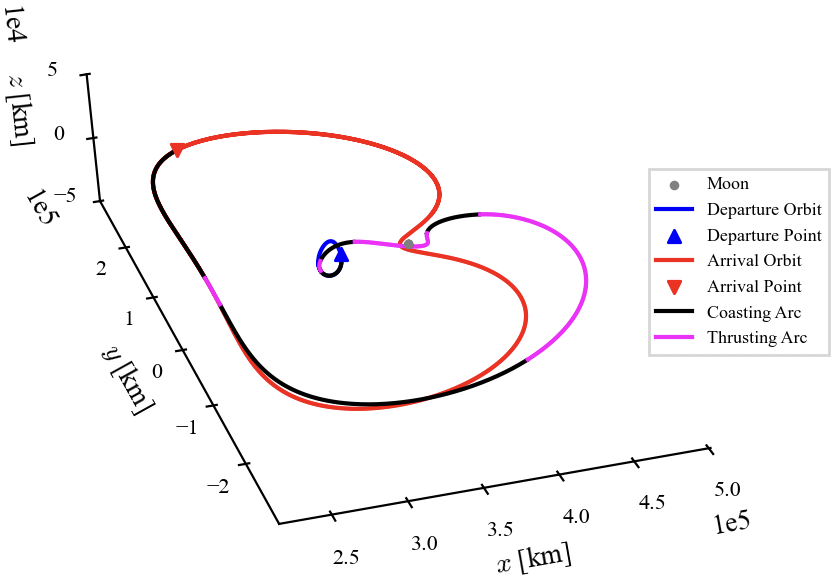
\includegraphics[width=0.75\linewidth]{Figures/truth_trajectory.png}
    \caption{Initial orbit, final orbit, and truth trajectory}
    \label{fig:truth_trajectory}
\end{figure}

\begin{table}
    \centering
    \begin{tabular}{c|c|c}
        Parameter & Value & Unit \\
        \hline
        $\rho$ & $10^{-4}$ & n.d. \\
        $\mu$ & $1.215059\times 10^{-2}$ & n.d. \\
        $u_\text{max}$ & $0.4$ & mm/s$^2$ \\
        $t_f$ & 35 & days \\
        $\sigma_\theta = \sigma_\phi$ & 0.001 & deg \\
        $\sigma_\text{scl}$ & 100 & n.d. \\
        $[\mu_0^{(1)}, \mu_0^{(2)}]$ & $[0.99, 0.01]$ & n.d. \\
        $\sigma_r(0)$ & $50$ & km \\
        $\sigma_v(0)$ & 1 & m/s \\
        $\sigma_{\lambda}(0)$ & 0.01 & n.d. \\
        $\Pi$ & $\begin{bmatrix}
            0.99 & 0.01 \\
            0.01 & 0.99
        \end{bmatrix}$ & n.d. \\
        $Q^{(1)}$ & $\begin{bmatrix}
            10^{-30}I_6 & 0  \\
            0 & 10^{-4}I_6
        \end{bmatrix}$ & n.d. \\
        $Q^{(2)}$ & $\begin{bmatrix}
            10^{-30}I_3 & 0 & 0 & 0 \\
            0 & 10^{-18}I_3 & 0 & 0 \\
            0 & 0 & 10^{-2}I_3 & 0 \\
            0 & 0 & 0 & 10^{-4}I_3
        \end{bmatrix}$ & n.d.
    \end{tabular}
    \caption{Simulation parameters}
    \label{tab:truth-parameters}
\end{table}

For a baseline, we compare the performance of the OCIMM to an IMM with assumed third order dynamics ($\bm{x} = [\bm{r}^\top, \bm{v}^\top, \hat{\bm{u}}^\top]^\top$) and two modes, a coasting and maneuvering mode. To make a fair comparison, the acceleration IMM also has knowledge of $u_\text{max}$, so its maneuvering mode is only estimating the direction of the control acceleration, $\hat{\bm{u}}$.

We perform simulations for two scenarios: one with measurements available at all time, and another with an artificial observation gap from $t \in [15, 20]$ days to assess the ability of the OCIMM to predict control. Each scenario is simulated with 100 Monte Carlo simulations. The parameters of the OCIMM and acceleration IMM are included in Table \ref{tab:truth-parameters}.

\section{Results}

To assess the estimation performance of the OCIMM, the mean absolute position, velocity, and acceleration errors of the OCIMM and acceleration IMM for the fully observed scenario are plotted in Fig. \ref{fig:MAE-normal}. In general, the OCIMM and IMM have similar MAE over the entire trajectory. The MAE of both filters spike at the beginnings and ends of maneuvers, as the truth control profile is bang-bang. The performance of the IMM and OCIMM differs at two times, which are during the flyby maneuver at $t \approx 10$ days and near the end of the third maneuver at $t \approx 20$ days. 

\begin{figure}
    \centering
    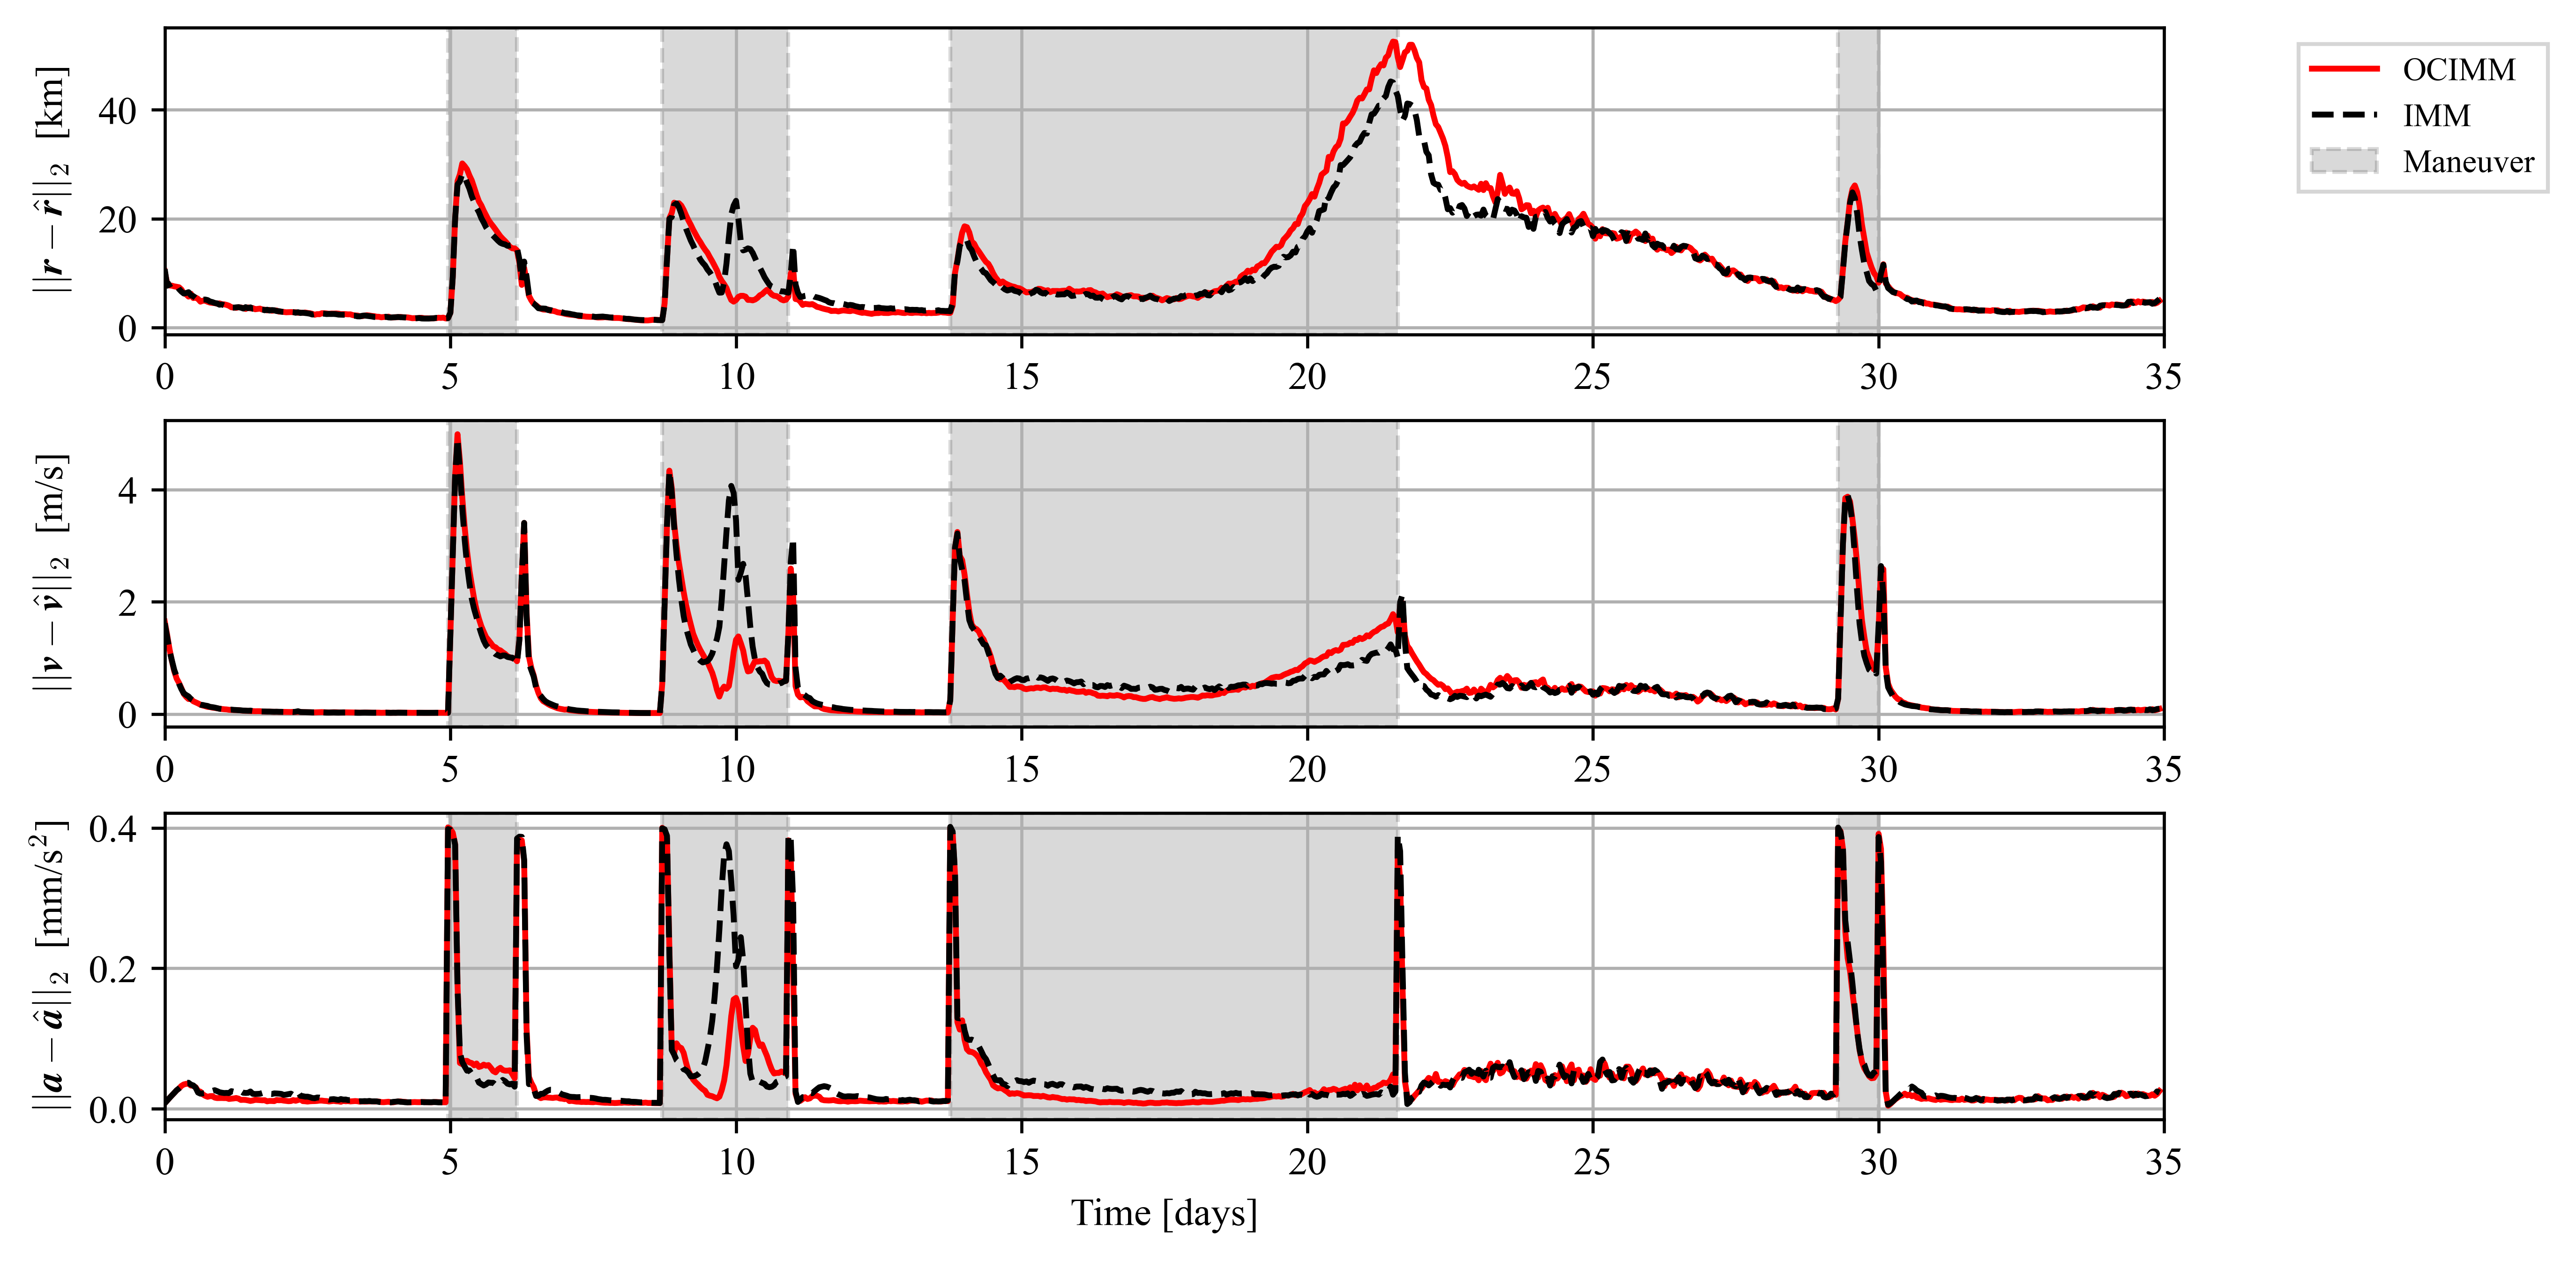
\includegraphics[width=1\linewidth]{Figures/MAE_normal.png}
    \caption{Mean absolute error of position, velocity, and acceleration estimates for fully-observed trajectory}
    \label{fig:MAE-normal}
\end{figure}

During the flyby maneuver at $t \approx 10$ days, the OCIMM outperforms the IMM. This is due to the high rate of change of the truth control. Because the OCIMM estimates the entire costate, it has some predictive power of how the control will evolve with respect to the state dynamics, so long as the true control is well-approximated by the OCIMM's assumed optimal control policy. In contrast, the IMM assumes that the control is constant (i.e. $\dot{\hat{\bm{a}}} = \bm{0}$), and so it has no predictive power, resulting in a lagging estimation during periods when the truth control has a high rate of change. The result is that the OCIMM outperforms the IMM during the flyby maneuver. 

Near the end of the maneuver starting at $t \approx 13$ days, the IMM begins to have slightly better MAE than the OCIMM. The reason for this is the OCIMM's overconfident estimate of the costates, which results in the filter "overpredicting" the control and being less receptive to measurement corrections. This could be solved by further tuning of the OCIMM.

Next, to test the performance of the OCIMM during observation gaps, the MAE of position, velocity, and acceleration of the OCIMM and IMM in the observation gap scenario are plotted in Fig. \ref{fig:MAE-gap}. During the observation gap from $t \in [15, 20]$ days, the OCIMM significantly outperforms the IMM. The reason for this is the ability of the OCIMM to predict the future control given some estimate of the current control. Since the observation gap occurs after the beginning of the third maneuver at $t \approx 13$ days, the OCIMM has been able to obtain some estimate of the costates given observations of the control. After the beginning of the observation gap, it is then possible to propagate the spacecraft under the assumed optimal control dynamics. This propagation is not perfectly accurate because the control $\bm{u}$ is only a function of $\bm{\lambda}_v$, so it is difficult to obtain an accurate estimate of $\bm{\lambda}_r$. Nevertheless, the general shape of the control profile is still accurately predicted by the OCIMM.

\begin{figure}
    \centering
    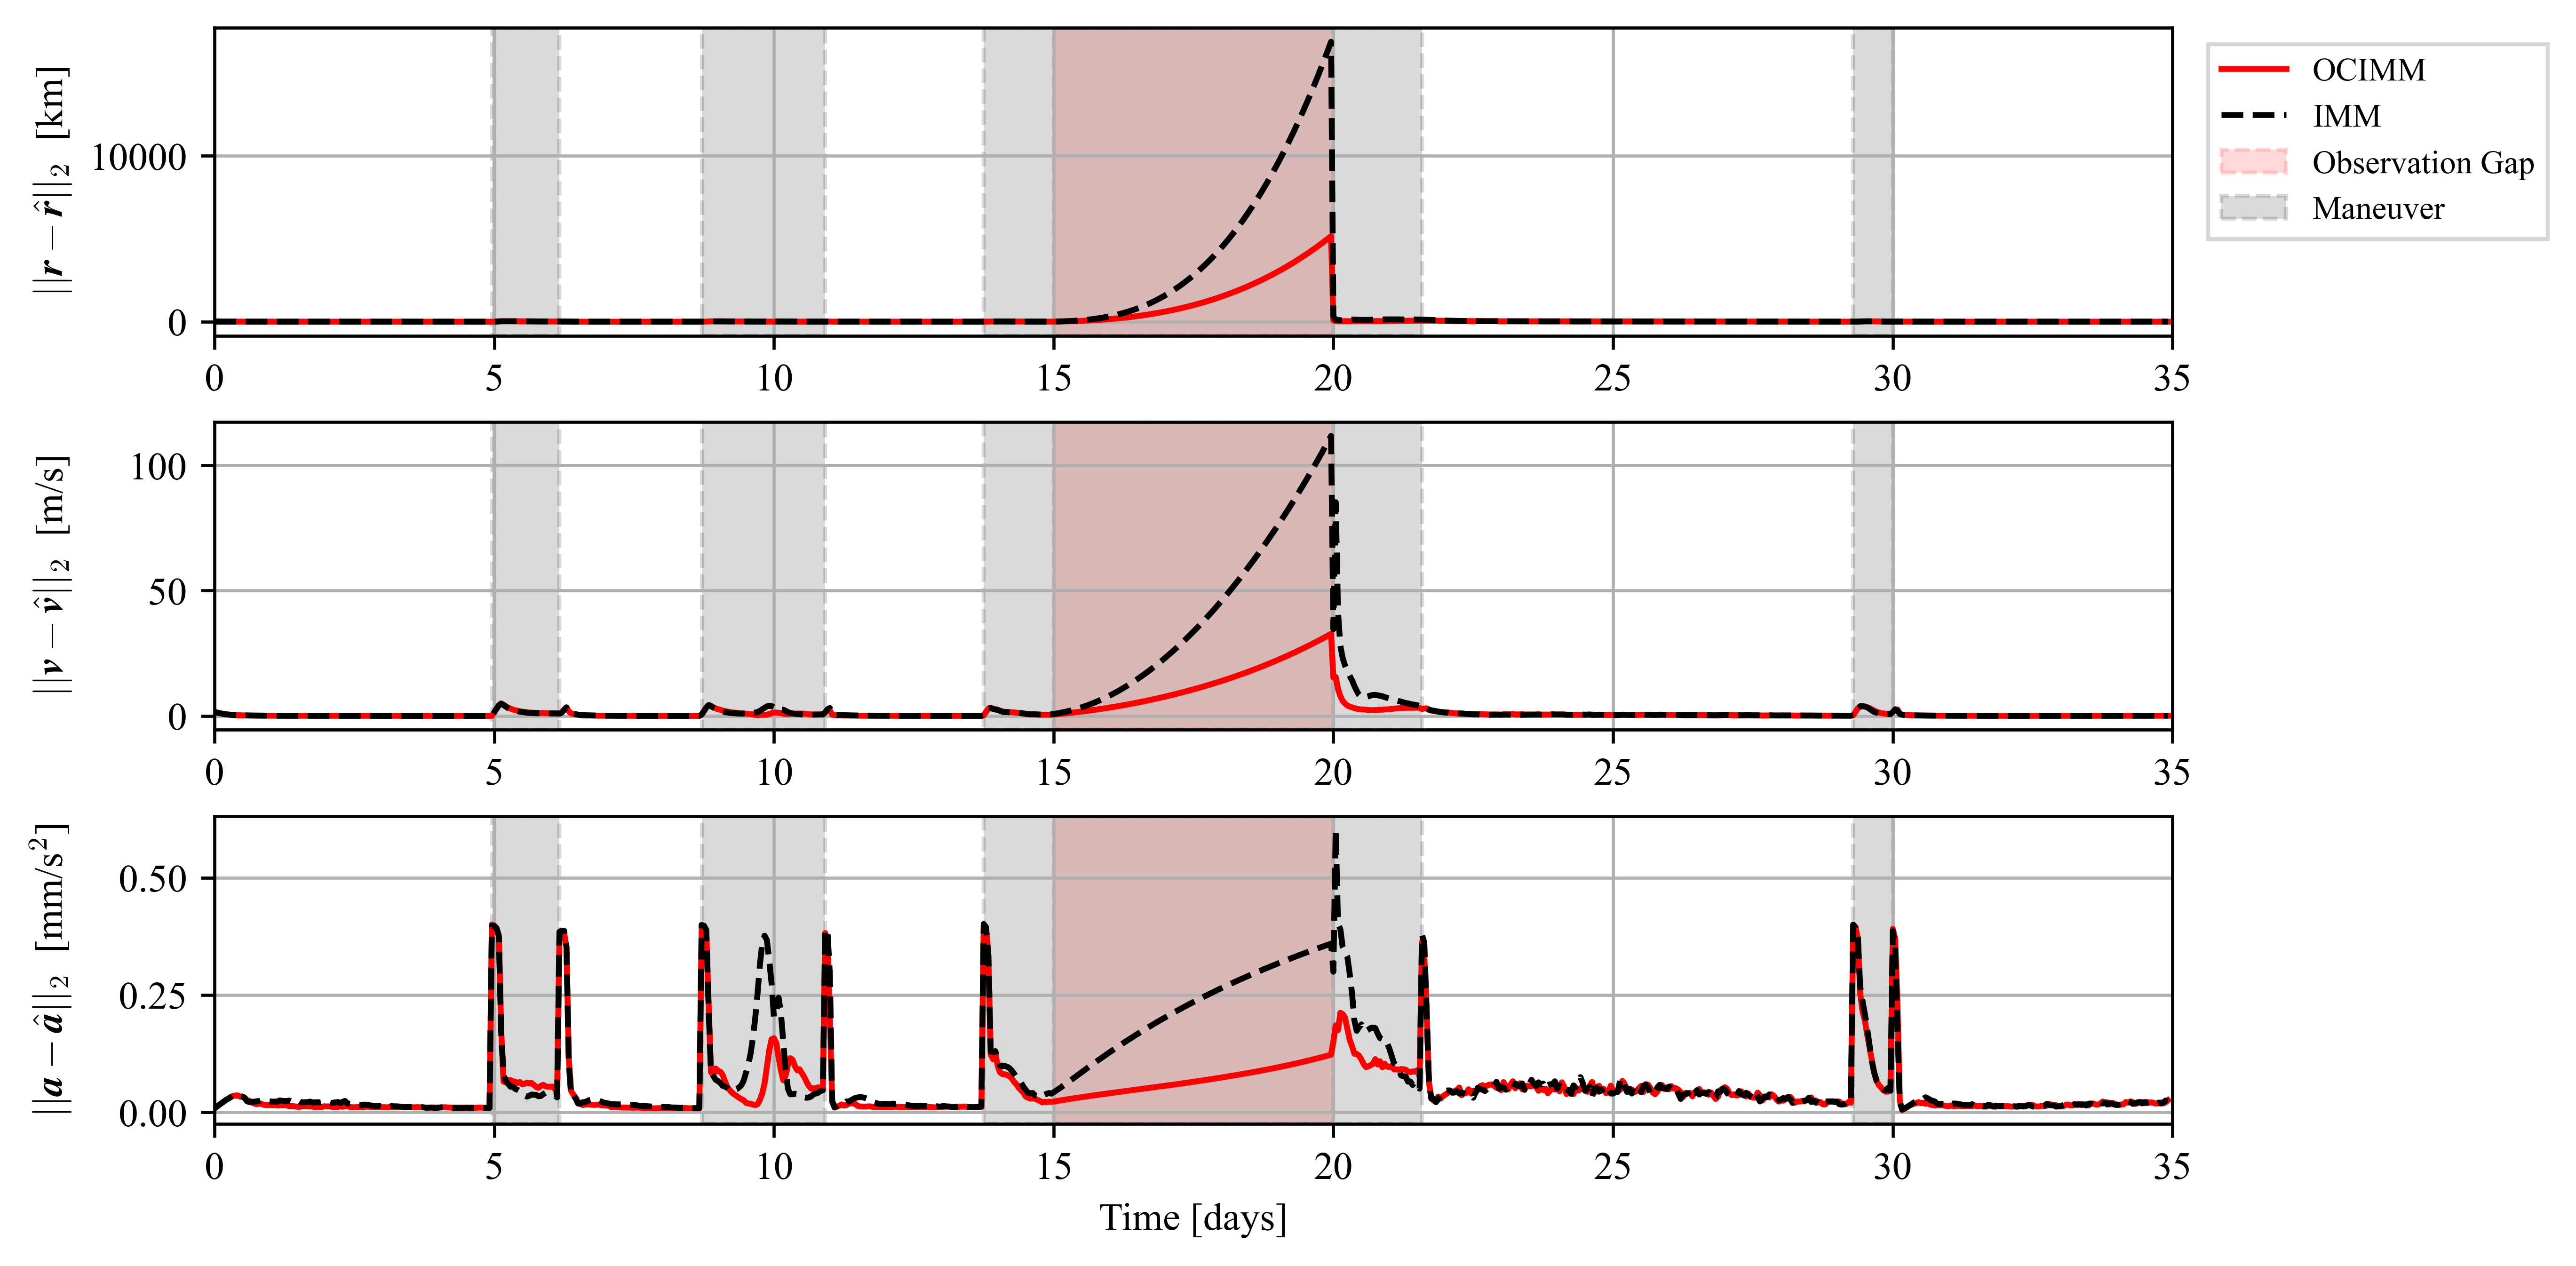
\includegraphics[width=1\linewidth]{Figures/MAE_gap.png}
    \caption{Mean absolute error of position, velocity, and acceleration estimates for trajectory with observation gap}
    \label{fig:MAE-gap}
\end{figure}

This predictive power is demonstrated by inspecting the assumed control of the OCIMM along with the truth control during the observation gap, plotted in Fig. \ref{fig:control}. Even after the beginning of the observation gap at $t=15$ days, the OCIMM is able to accurately estimate the general shape of the truth control because of the inclusion of optimal control in its maneuvering mode dynamics.  

\begin{figure}
    \centering
    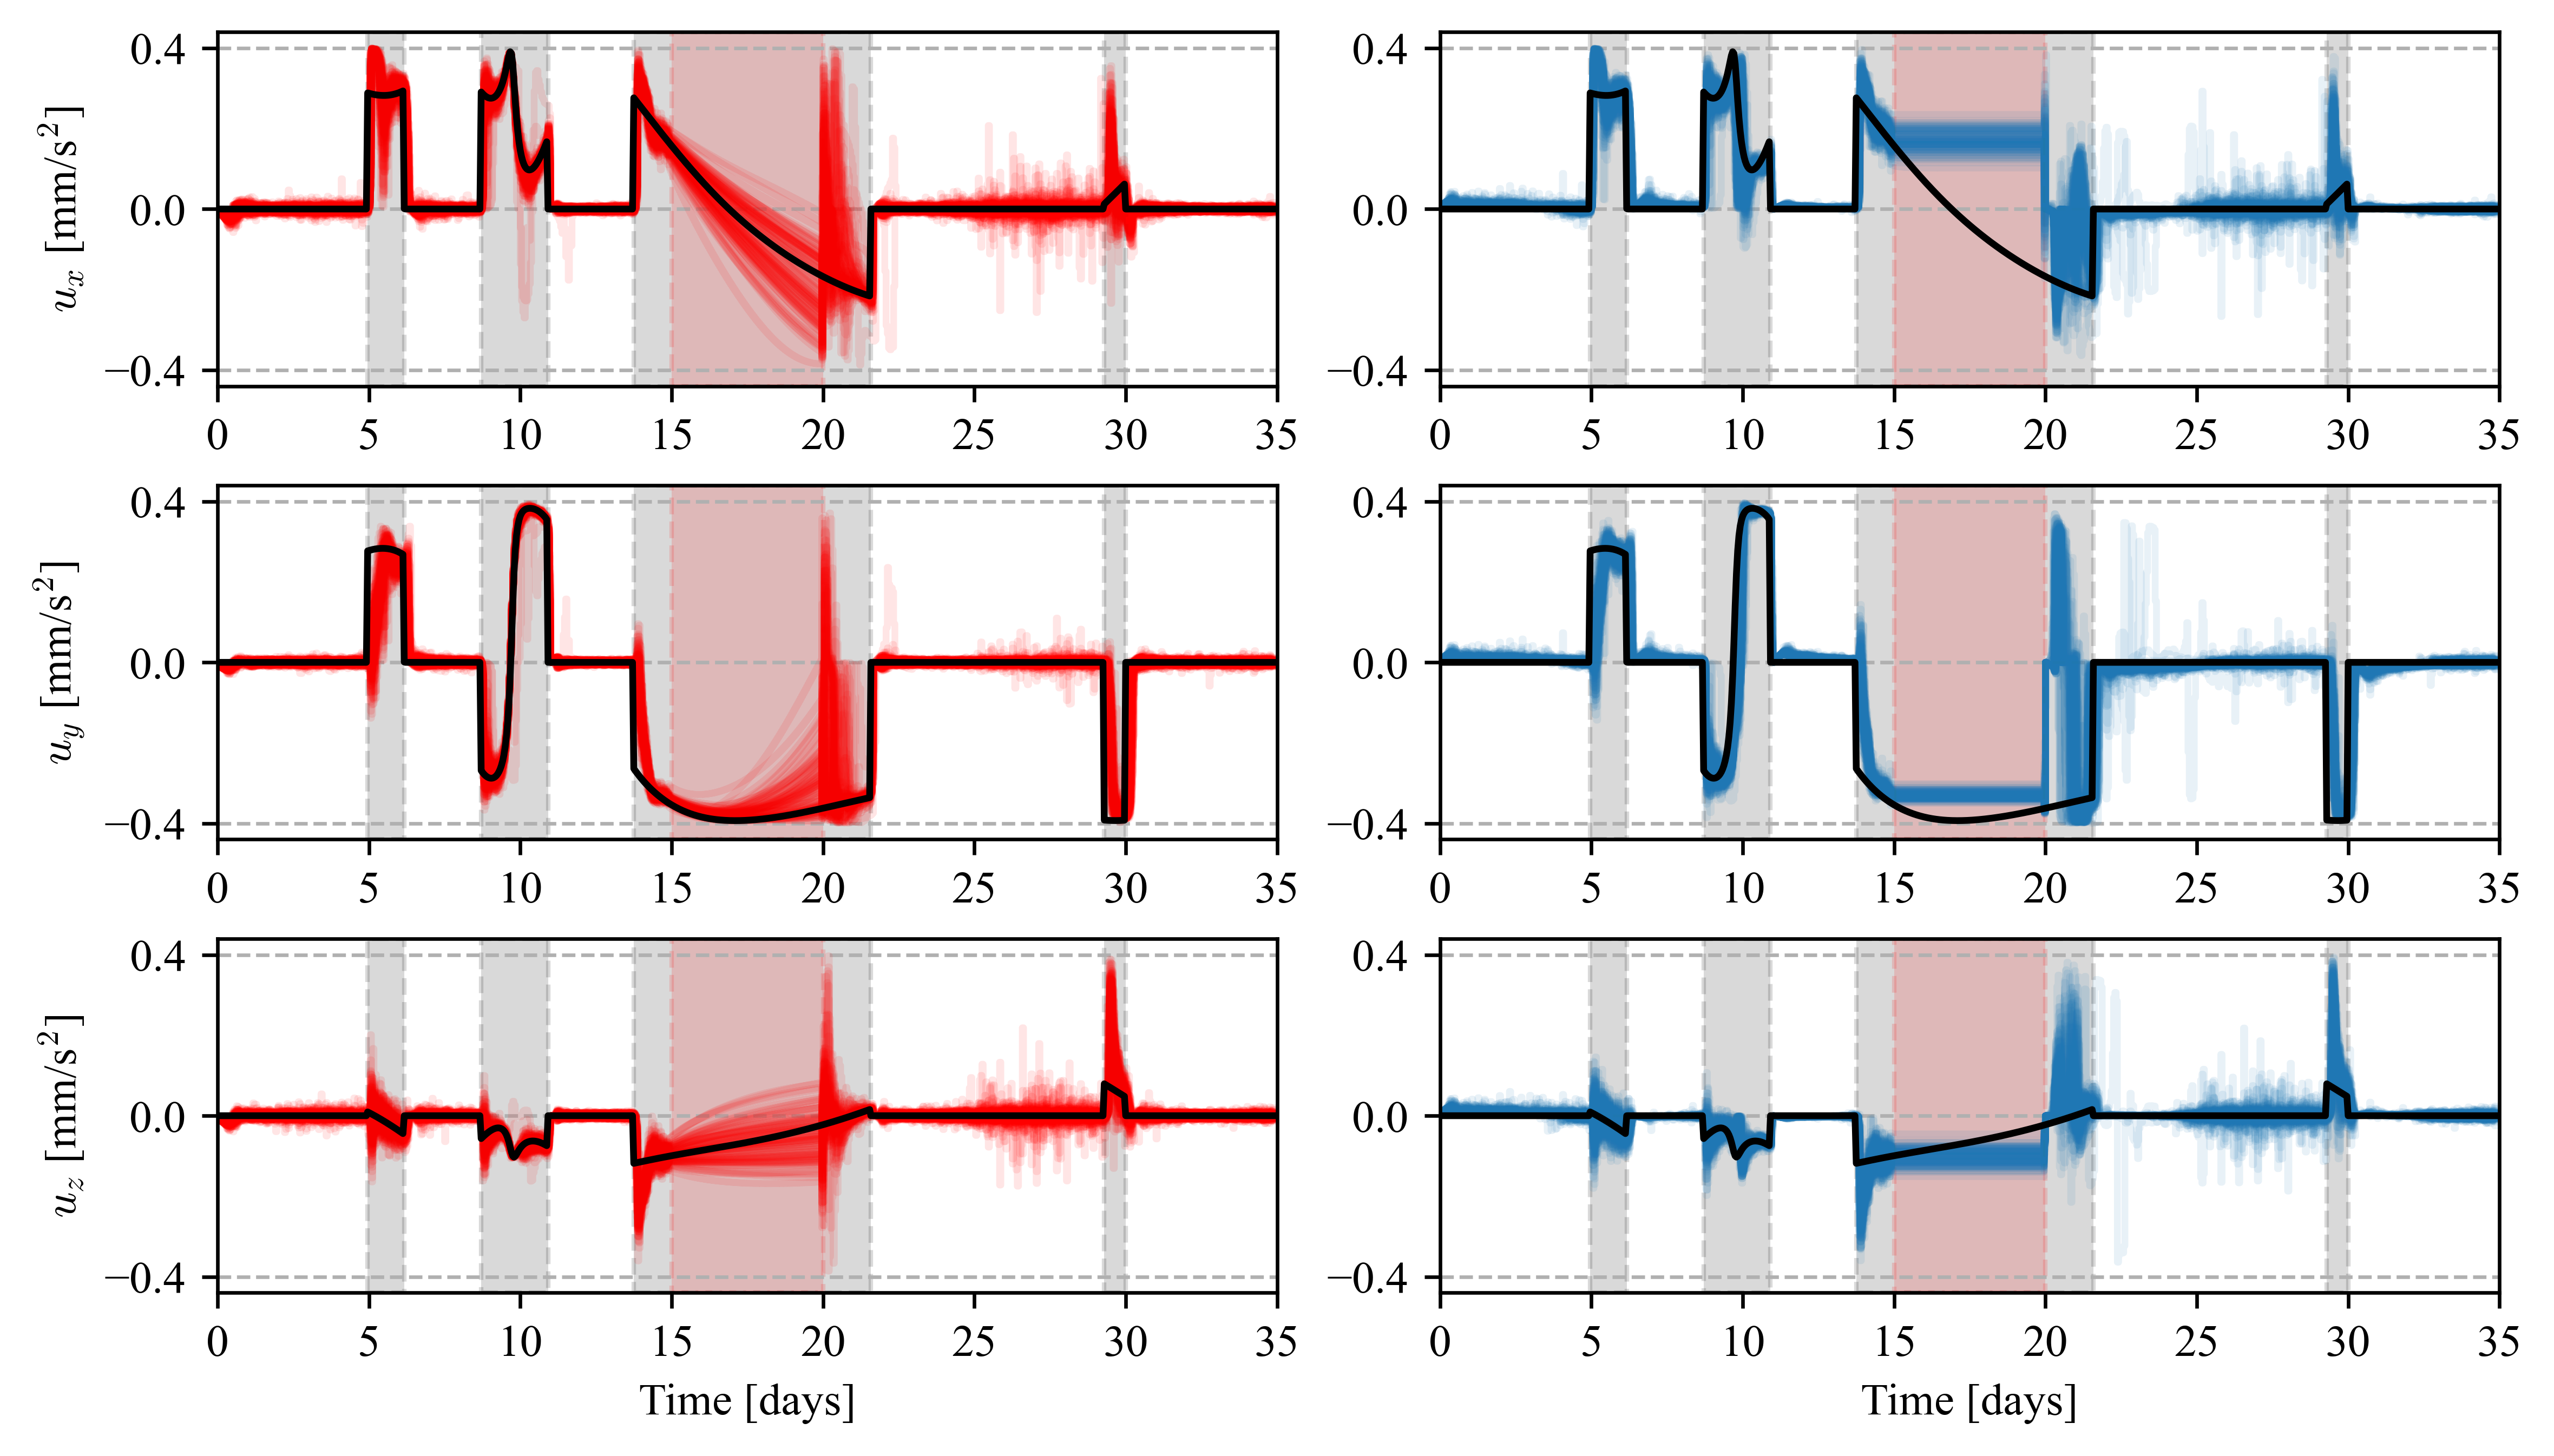
\includegraphics[width=1\linewidth]{Figures/control.png}
    \caption{Estimated control of OCIMM over 100 Monte Carlo simulations for trajectory with observation gap}
    \label{fig:control}
\end{figure}

Lastly, to assess the consistency of the OCIMM, its estimation error and estimation error $3\sigma$ values from the observation gap scenario are plotted in Fig. \ref{fig:three-sigmas}. Since the OCIMM is estimating the costate, the covariance of the control must be obtained by linearly transforming the costate covariance. This transformation is described in Eq. \ref{eq:covariance-transform}:

\begin{align}
    P_{u, k} = U_kP_{\lambda_v, k}U_k^\top, \quad U_k = \left. \frac{\partial \bm{u}(\bm{\bm{\lambda}})}{\partial{\bm{\lambda}}} \right|_{\bm{\lambda}=\bm{\lambda}_k}, \quad \bm{u}(\bm{\lambda}) = -u_\text{max} \frac{\bm{\lambda}_v}{\norm{\bm{\lambda}_v}_2} \label{eq:covariance-transform}
\end{align}

\noindent It can be seen that the OCIMM is able to maintain convergence when directly estimating the costate, even in periods of rapidly changing control and after observation gaps. This demonstrates the validity of an estimation approach which directly implements the costate in the state vector. 

\begin{figure}
    \centering
    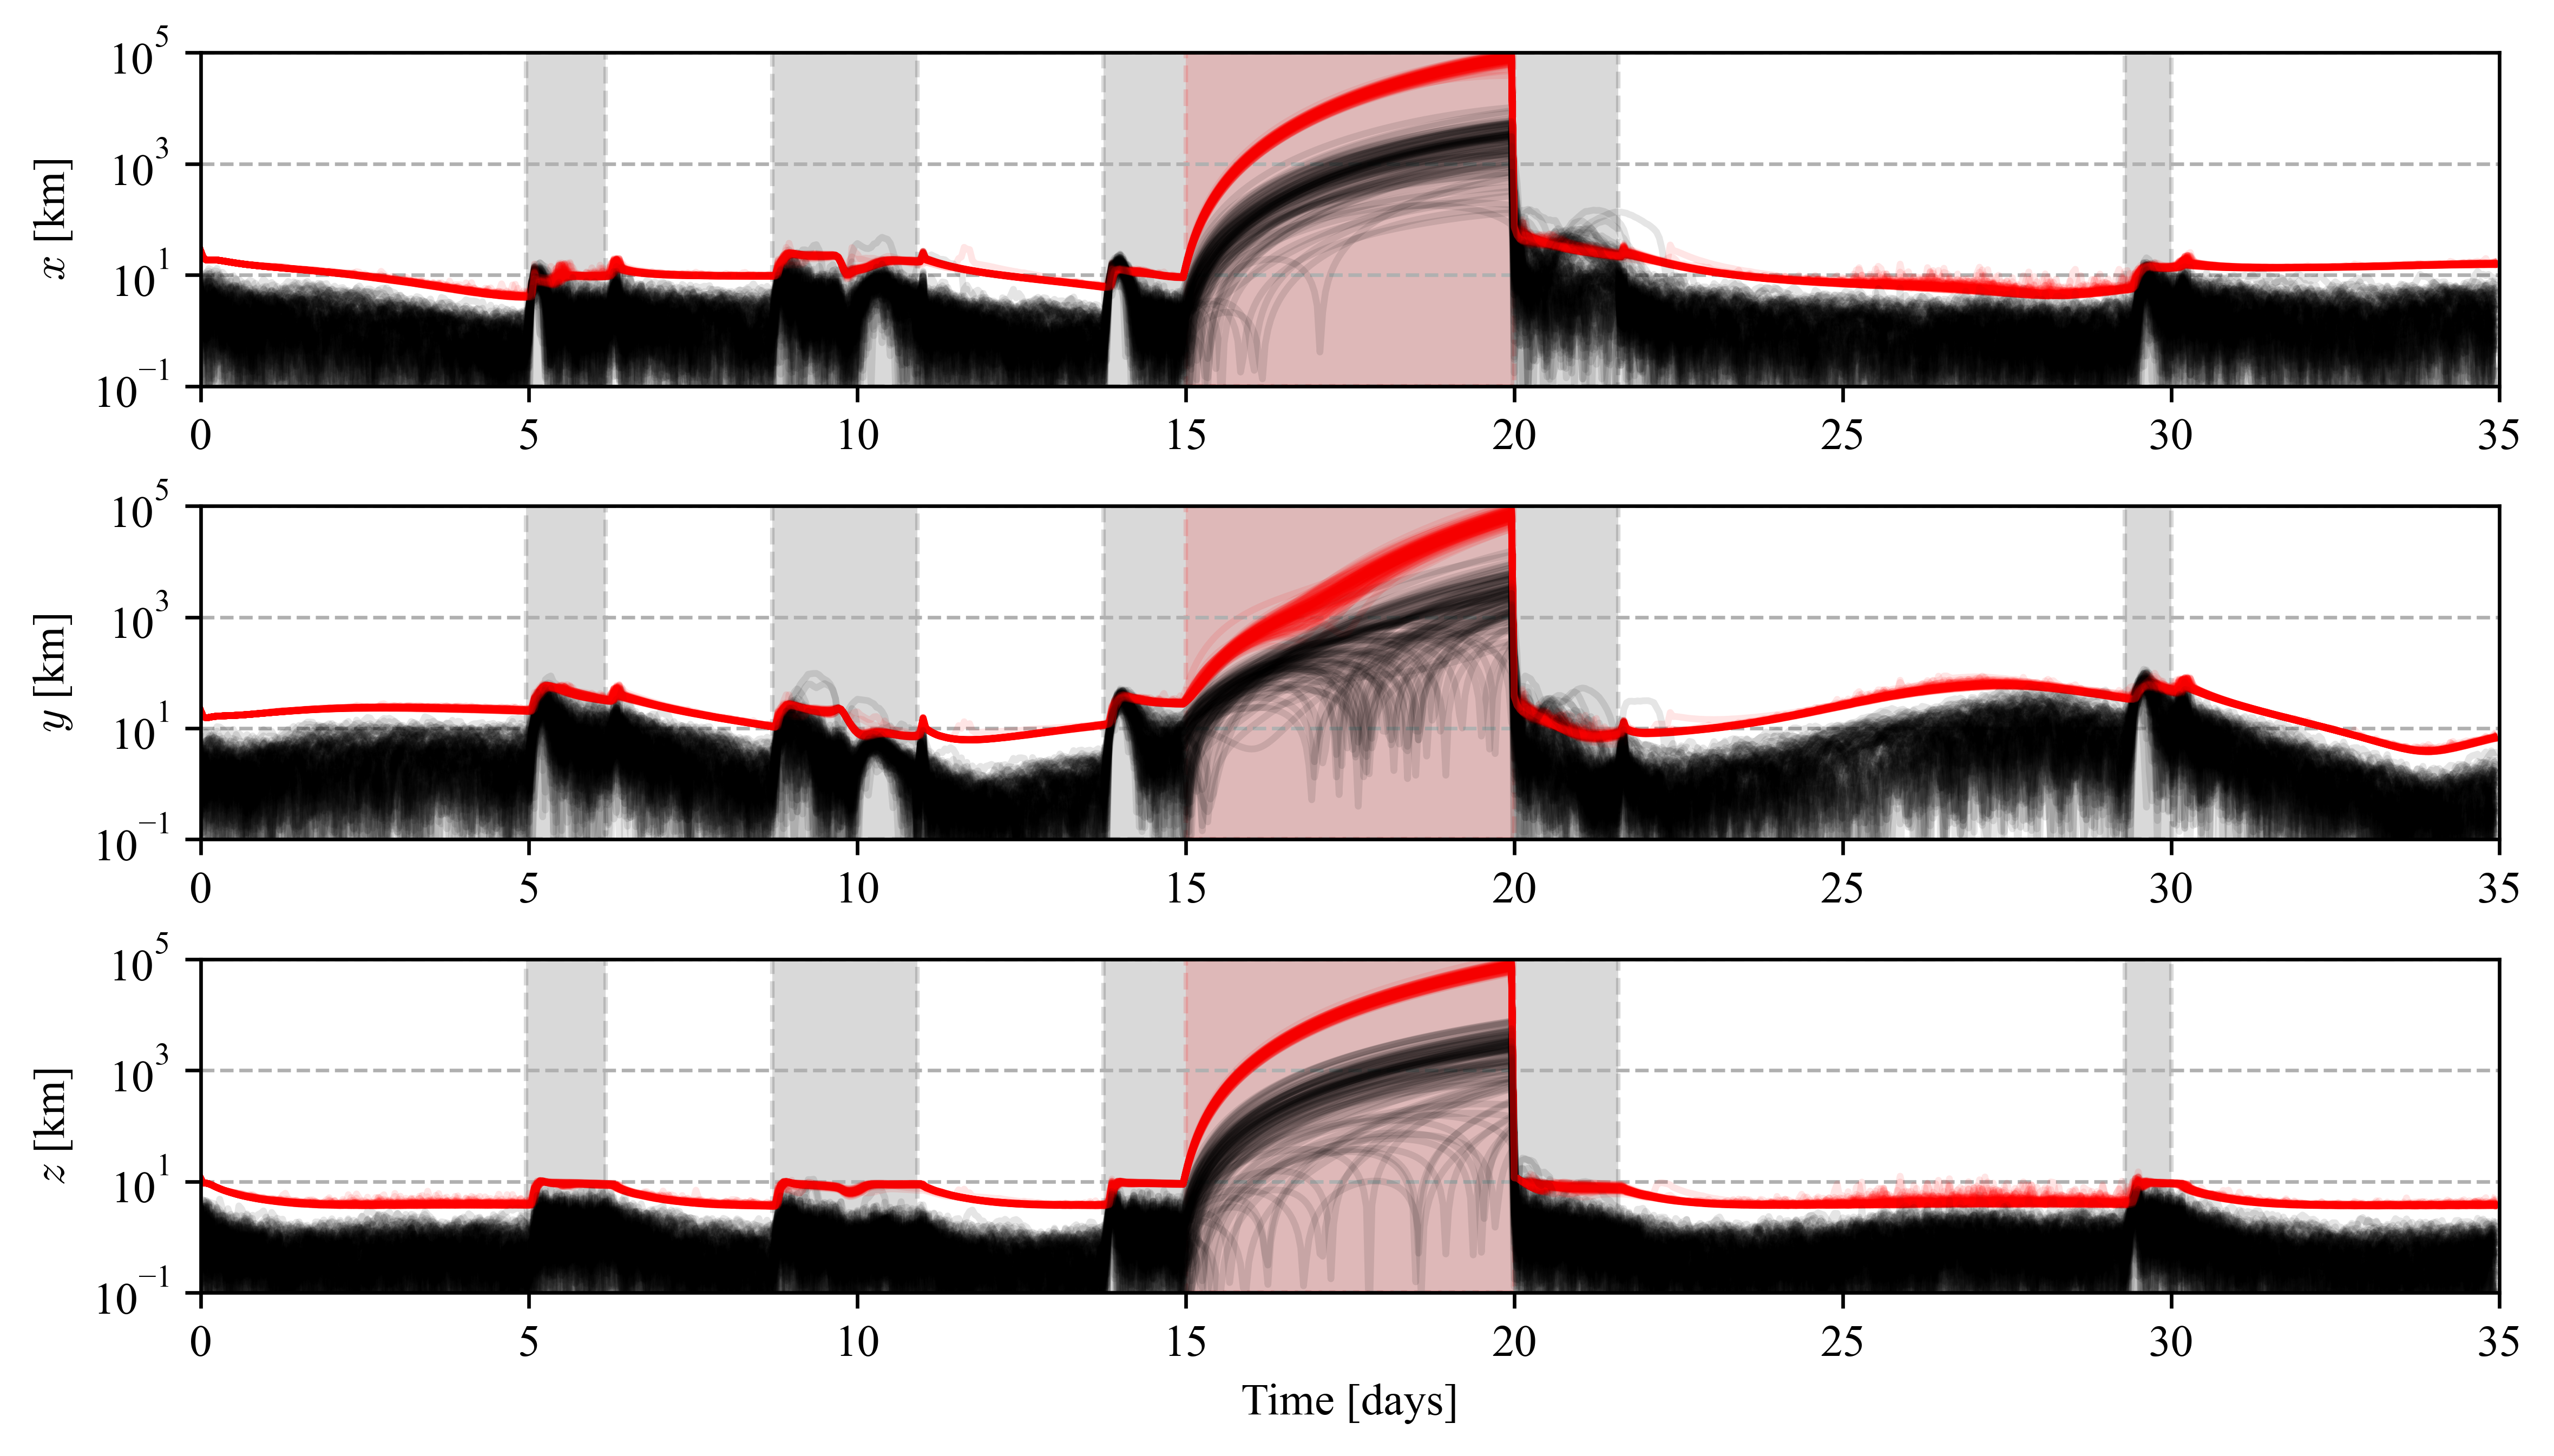
\includegraphics[width=0.9\linewidth]{Figures/position_3sigmas.png}
    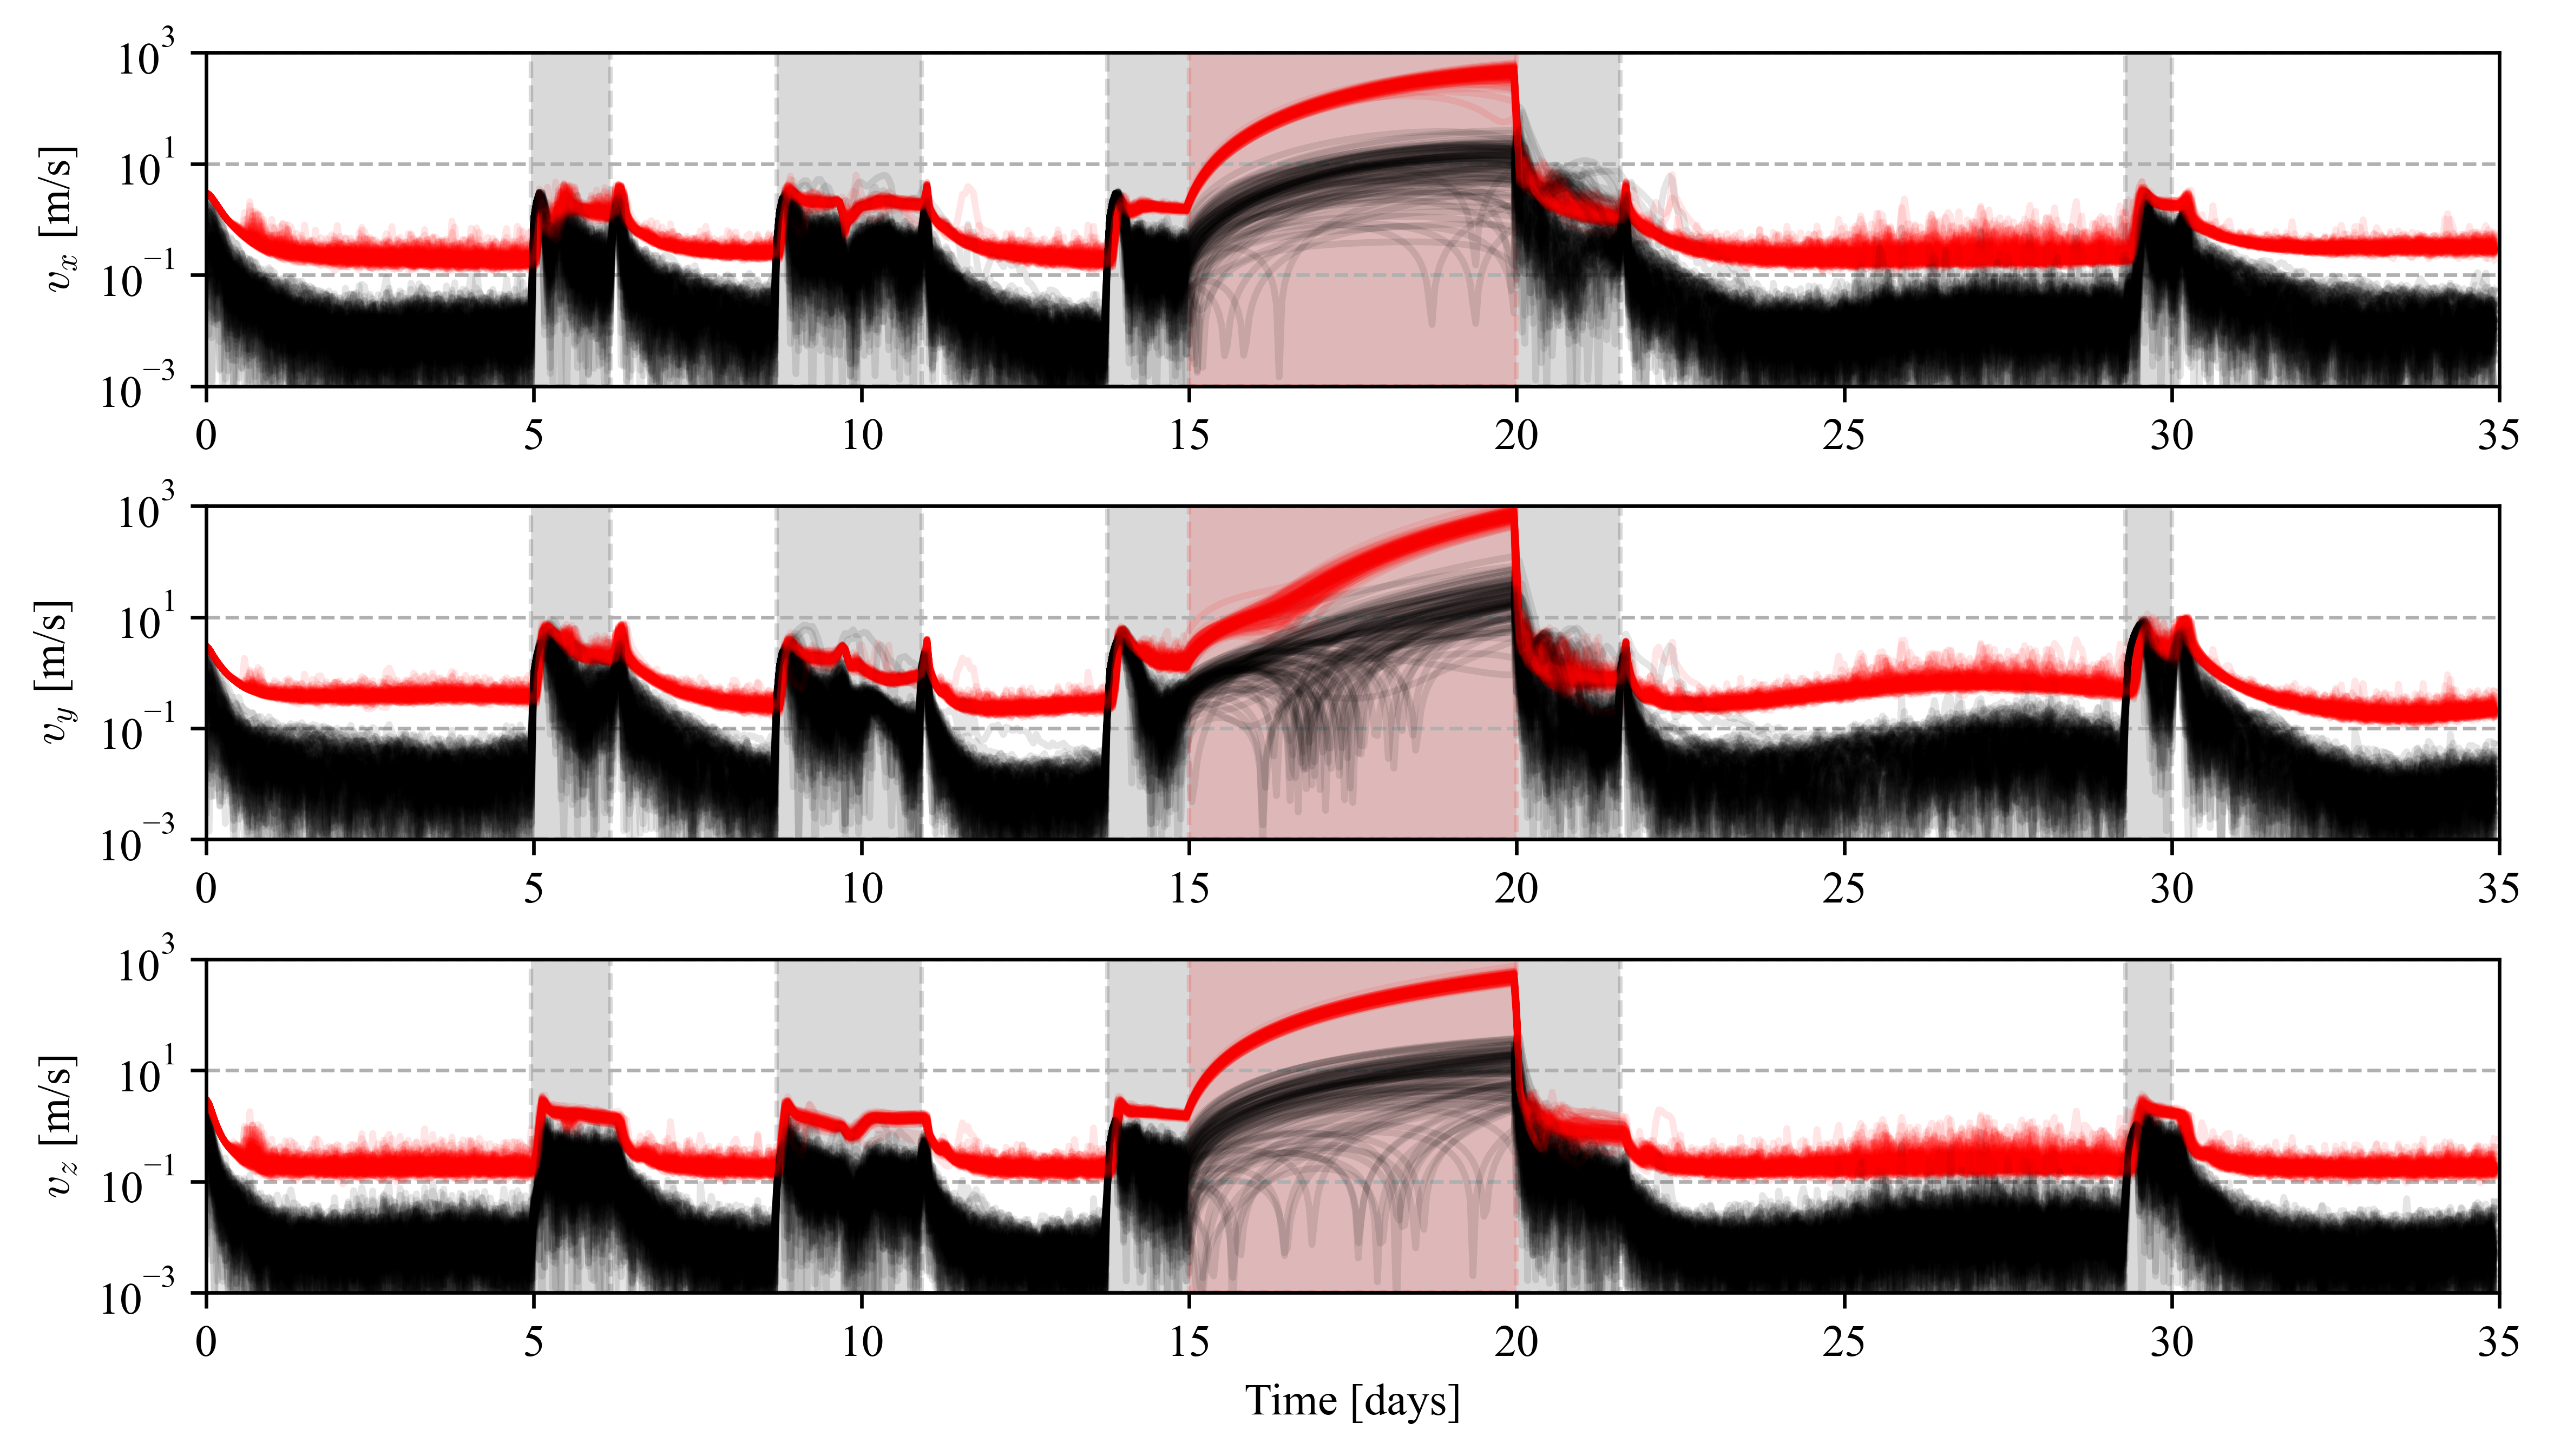
\includegraphics[width=0.9\linewidth]{Figures/velocity_3sigmas.png}
    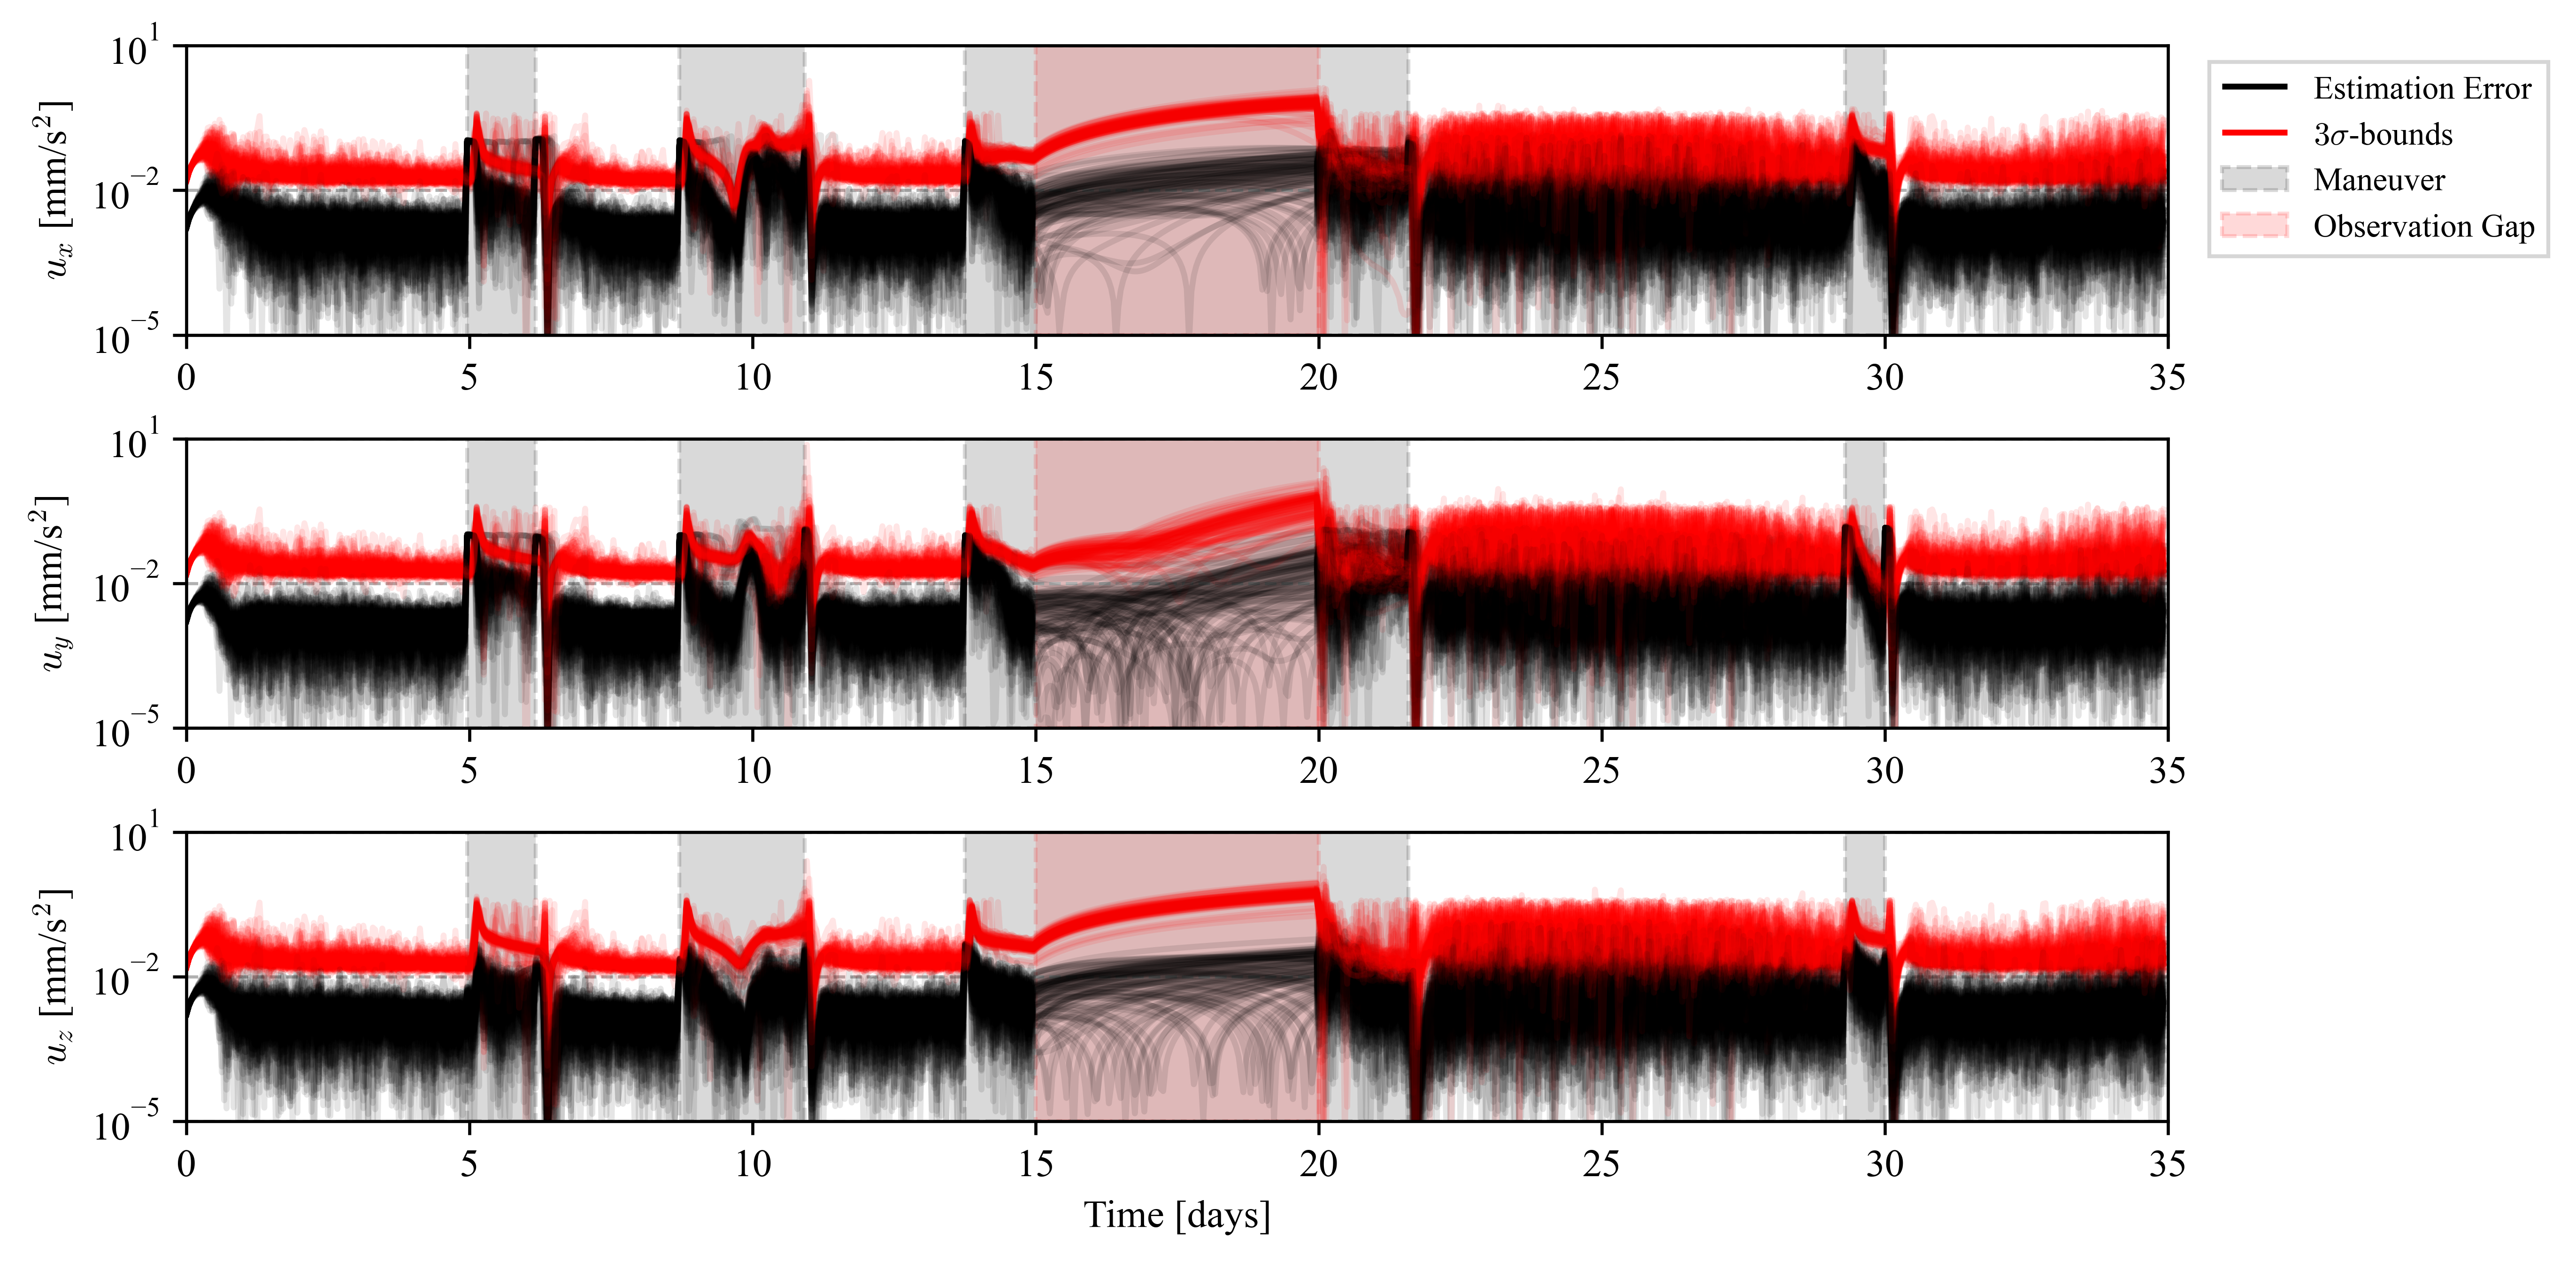
\includegraphics[width=0.9\linewidth]{Figures/control_3sigmas.png}
    \caption{Position, velocity, and control estimation errors and estimation error $3\sigma$ values for the OCIMM over 100 Monte-Carlo simulations}
    \label{fig:three-sigmas}
\end{figure}

\section{Conclusion}

This paper presents the tracking of a low-thrust, maneuvering spacecraft in cislunar space with the implementation of an assumed optimal control policy directly into a sequential filter through the application of Pontryagin's Minimum Principle. The resulting optimal control IMM (OCIMM) is able to accurately predict the control input of a low-thrust maneuvering spacecraft in cislunar space maneuvering under an bang-bang, fuel-minimum control policy, even in the presence of rapidly changing control inputs and observation gaps. This predictive power results in superior performance compared to a traditional acceleration IMM. 

There are several opportunities to improve the presented work. Additional models can be implemented into the IMM to simultaneously account for more possible control policies, as the current implementation assumes only a single optimal control policy. Principles of the variable state dimension filter can be implemented to account for the estimation error spikes at the starts and ends of coasting arcs while also allowing for a more accurate initial guess of the costate at the beginning of maneuvers. Finally, the presented work assumes that the maximum acceleration of the spacecraft $u_\text{max}$ is known, so an improved estimator could be designed to simultaneously estimate this maximum thrust along with the spacecraft states and costates. 

\bibliographystyle{AAS_publication}   % Number the references.
\bibliography{references}   % Use references.bib to resolve the labels.



\end{document}
